%% @author Y.Chevallier <me@yves-chevallier.com>
%% @language LaTeX2e
%% @date Jan 2012
%% --------------------------------------------------------------------------
\documentclass{kepfl}
\usepackage[small,bf]{caption}
\usepackage{glossaries}
\usepackage{appendix}
\usepackage{rotating}
\usepackage{morefloats}
\usepackage{cellspace} 
\makeglossaries
\lstset{%
language=C,
breaklines=true, 
breakatwhitespace=false, 
basicstyle=\footnotesize}

%\renewcommand{\tabularxcolumn}[1]{S{m{#1}}} 
\newcolumntype{T}[1]{>{\hsize #1\hsize}X} 
\newcolumntype{M}[1]{>{\hsize #1\hsize\centering}X} 
\newcolumntype{L}[1]{>{\hsize #1\hsize}X} 
\def\tnl{\crcr \hline }

\makeindex

\newglossaryentry{nus}{name=NUS, description={National University of Singapore}}

\begin{document}

%% Define title page
%% --------------------------------------------------------------------------
\pagenumbering{empty}
\date     {\today}
\author   {Yves Chevallier \\ Project completed at SMART Singapore}
\title    {Holographic Optical Tweezers for a \\Volume Hologram Imaging Application}
\subtitle {Master's Thesis 2011-2012}
\teacher  {Prof. C. Moser (EPFL)\\
	   Prof. G. Barbastathis (MIT)\\
	   Prof. Y. Luo (National Taiwan University)}
\maketitle
\newpage
\setlength{\parskip}{1em}
\frontmatter 

%% Acknowledgements
%% --------------------------------------------------------------------------
\begin{acknowledgements}
I would like to thank my supervisor Prof. Yuan Luo from National Taiwan University for his help and continued supervision during my project. 

I am heartily thankful to Chen Zhi, for his encouragement, guidance and support throughout my work at SMART. 

Also many thanks to Prof. George Barbastathis and Prof. Christophe Moser for allowing me to pursue a project in a subject that is relevant to my interests. 

Lastly I offer my regards and blessings to Sijia and all those who have supported me in any respect during this master's project. 
\end{acknowledgements}
\clearemptydoublepage

%% Abstract page
%% --------------------------------------------------------------------------
\begin{abstract}
% English
The Singapore-MIT Alliance for Research and Technology (SMART) and the Massachusetts Institute of Technology (MIT) have developed new imaging techniques for multi-plane imaging and phase retrieving for transparent objects. The objective is to assess the feasibility for three-dimensional reconstruction of biological cells with projected tomography. In order to achieve this, a proposal for using optical tweezers has been suggested. Nonetheless, SMART lacked adequate knowledge in this area. This master's project is an opportunity to explore this area and develop new skills with optical trapping. 

\vspace{1em}
\asterism
\vspace{1em}

% French
L'alliance MIT-Singapour pour la recherche et la technologie (SMART) ainsi que le  Massachusetts Institute of Technology (MIT) ont d�velopp� une nouvelle technique d'imagerie � plusieurs plans permettant la reconstruction d'objets de phase donc pratiquement transparents. Ils souhaitent � pr�sent d�montrer la faisabilit� d'une reconstruction en trois dimensions, par tomographie, de cellules biologiques en utilisant des pincettes optiques, un domaine encore peu connu de ces groupes de recherche. Ce projet de master est une chance pour acqu�rir de nouvelles comp�tences dans ce domaine. 

\end{abstract}

%% Table of contents, list of figures and tables and glossary
%% --------------------------------------------------------------------------
\clearemptydoublepage
\tableofcontents
\clearemptydoublepage
\pagenumbering{arabic}

%% Content
%% --------------------------------------------------------------------------
\mainmatter
\chapter{Introduction}
\maraja{Microscopy, in perpetual growth}
Microscopy imaging techniques belong to a growing industry and research in this domain continues to be active. Therefore, there exists a significant need for better images. Besides wanting to see deeper \emph{in vivo}, biologists want to get a wider field of view and acquire images faster. But above all, they covet a better overall view of their samples. Nowadays, three-dimensional \index{3D} imaging techniques for living objects are rather limited to the amplitude component of light in the domain of visible wavelengths. An organic cell is usually a transparent object which affects almost only the phase component of light. With this in mind, many researchers are attempting to use advanced optical techniques to retrieve phase information to make visible the invisible and with this, offer more suitable instruments to enhance research in life sciences.  

\maraja{SMART built a promising apparatus for multi-plane phase imaging}
In 2010, SMART and MIT developed a new Volume Holography Imaging System (VHIS) \cite{VH}. With the benefit provided by the Transport Intensity Equations (TIE)\index{TIE} \cite{TIE-Diamond}, phase biological samples can be imaged on different planes simultaneously. It means neither the imaging system nor the sample need to be moved to get images at different depths. Moreover, an assumption is made the imaging system is telecentric and the depth of focus is high with regards to the object size, different cross-section projections can be obtained by rotating the sample along an axis normal to the imaging direction and relative to a fixed point. Using standard tomography techniques, a three-dimensional representation of the object can subsequently be reconstructed with the data acquired. 

\maraja{Optical Tweezers, favored for rotation}
With this in mind, the Center for Environmental Sensing and Modeling (CENSAM) based in Singapore is now looking for a method to enable the rotation of a transparent microscopic sample with precise control of the angle. Optical tweezers pioneered by Askin in 1986 have been increasingly used for micro-manipulation and particularly for biological objects in order to study the varied biological processes. A highly focused laser beam going through the objective of a regular microscope can trap, move and rotate micrometric scale objects. 

\maraja{Towards a new publication?}
SMART has previously published promising results of projected tomography of a transparent sample using TIE. More than that, TIE was successfully combined with a VHIS to retrieve phase information of an organic sample. Using these results to achieve tomography is a new step which is yet to be demonstrated.  

\maraja{Acquire the knowledge}
Using optical tweezers to rotate an biological specimen seems more complex to implement than using a conventional rotational microstage, but SMART wants to assess the feasibility of this technique and at the same time acquire the knowledge of optical trapping. In any case, tomography using a conventional rotation technique has already been done by Mark Fauver and Eric J. Seibel in 2005 \cite{FAUVER2005}.
 
Consequently, this project is above all an attempt to bring the expertise of optical tweezers and holographic optical tweezers to SMART

\maraja{Master's project}
Prof. Christophe Moser from EPFL in Lausanne, Switzerland contacted Prof. George Barbastathis of MIT 3D Optical Systems Group, in Boston, U.S., for my participation in this project to pursue my master's thesis. I was invited to work for 25 weeks in Singapore under the responsibility of SMART and CENSAM, and to collaborate in a team with Chen Zhi and Wensheng Chen and Prof. Yuan Luo. 

\section{Context}
\maraja{Projected Tomography}
Tomography is a major imaging technology that allows for three-dimensional reconstruction by sectioning an object using a penetrating wave. Projected Tomography like Computed Tomography (CT) uses X-rays to obtain an image projection through the matter. Often, the target or the imaging instrument needs to be rotated along a fixed axis in order to obtain multiple image projections. The post-treatment requires sophisticated algorithms including the Radon transform that allows building of a three-dimensional view from the cross-sectional scans of the object. 

In the microscopic world, Electron Tomography is the only available method to image structures such as bacteria, biological cells or body tissues. An electron beam crossing the sample is partially absorbed depending on its composition. A sensor placed after the sample retrieves the cross-sectional projection for each angle. However this technique cannot be applied with a living specimen. The object needs to be scanned at a low temperature and this process takes time. 

%\figc{ET}{Electron Tomography principle}{Electron Tomography principle. (a) Projected tomography with microscope and (b) Projected electron tomography with glass tube containing the sample.}

\maraja{TIE for phase retrieval}
Three-dimensional imaging techniques in the visible range belong to a growing field, which is in intense development in research. SMART wants to leverage its volume holography system with the transport intensity equations to obtain three-dimensional images from biological phase objects. TIE Tomography already demonstrated promising results by showing a 3D-reconstruction of a Pyrex diamond placed in an index-matching fluid \cite{TIE-Diamond}. Figure \ref{tie} illustrates some of the published results.

\figc{tie}{TIE Tomography}{Principle of TIE Tomography showing in (a) a simple image in focus of the diamond immersed. (b) TIE phase retrieval from two images out of focus. (c) Three-dimensional reconstruction of the phase object obtained with Radon transform}

\maraja{VHIS for imaging}
The Volume Holographic Imaging System uses a thick hologram to record different two-dimensional planes located at different depths simultaneously without scanning. Each plane appears as a vertical narrow band on the camera plane. By varying the type of grating of the hologram, it is possible to obtain a different number of planes with a defined spacing between each plane.  Figure \ref{vh} shows the type of image we can expect to obtain with this system. 

\figc{vh}{VHIS Images}{VHIS Imaging, (a) Onion skin, 5 planes, (b) 3D stack of image a (c) Mouse fat, 2 planes}

\maraja{VHIS + TIE for tomography}
As TIE requires at least two out-of-focused images slightly above and before the object to reconstruct the phase information, VHIS provided a suitable solution to obtain these images simultaneously. In 2010, Laura Waller and co-workers combined these two techniques \cite{TIE-VH} and showed promising results. Now, Prof. Yuan Yuo from the National Taiwan University would like to take a step further to achieve tomography of biological phase objects with a volume holographic imaging system and in combination with the transport intensity equations. This is something which has not been done before. 

\maraja{But we still need to rotate}
Providing a demonstration of the feasibility of this technique could offer a versatile solution for imaging living cells in the micrometric scale. However, in order to reach this objective, the rotation of the specimen must be perfectly controlled first.  

\maraja{Optical Tweezers for rotation}
Optical tweezers have proven their capabilities for moving, stretching and rotating microscopic living objects. A significant number of research groups have designed different solutions to rotate such objects. For example, in 2008, M. K. Kreysing \emph{et al.} from the University of Leipzig, Germany, used a modified dual-beam laser trap delivered by two optical fibers to rotate a red blood cell around an axis perpendicular to the optical direction \cite{KREYSING2008}. Nevertheless, this solution is challenging to implement and is not very versatile because the alignment of the two fibers are critical. Therefore, this project will focus on the rotation of micro-organisms with standard optical tweezers. 

\clearpage
\section{Project goals}
Unlike other EPFL masters' projects, this project did not begin with specified goals. As with a research project, the objectives were changed many times following our weekly team meetings. As below are some of the goals which were eventually set in place:

\begin{enumerate}
\item Explore state-of-the-art techniques in optical trapping
\item Build a conventional optical tweezers system
\item Allow multi-trapping
\item Achieve rotation of particles
\item Build a volume hologram setup 
\item Combine optical tweezers with the volume hologram system
\item Move particles simultaneously on different planes of the VH system
\item Obtain image and results
\item Propose a solution for rotation of biological samples
\item Propose further investigations
\end{enumerate}

As required by EPFL, this master's project will last for 25 weeks starting from September 17, 2011. The final report has to be submitted by the noon of March 16, 2012 and the oral presentation is scheduled to take place in early April . 

The first part of this project consists of learning about the state-of-the-art techniques in optical trapping. Many recent publications show interesting applications. Multi-trapping not only requires a good knowledge of digital holography and light propagation but also requires a practical experience of spatial light modulators and optical components. 

The second part deals with the volume hologram setup. The alignment of this system is very sensitive and every component has to be assembled carefully. In addition, compromises must be made to combine the volume hologram system with the tweezers setup due to their stringent requirements. 

Finally, a solution must be designed so that the biological samples can be precisely rotated from the imaging axis. The potential problems encountered will be recorded in order to allow for further investigations. 
 
\clearpage
\section{Organization}
This report is mainly divided into two parts. The first part is a theoretical approach of optical trapping, volume holography and micro-fabrication based on scientific publications and books. Most of the illustrations found in this document are inspired from these readings but they were redrawn for better understanding and a better consistency. The second part is focused on experiments where results and issues are shown and explained. This part ends with a discussion of the results and suggests the possibility of further investigations. 

This report is not intended in any way to be published because its content relates scientific material which may be misused for competing on a scientific basis. In contrast, this report must be considered as a knowledge base for the continuation of this project. It reports the experience, the results and the thoughts acquired during this work. 

\todo{Why not adding a section ``Lecture convention'' with explanations of side page notes, typography conventions, general structure. Maybe this can complete this almost empty page\ldots}

\chapter{Optical Trapping}
\section{Introduction}
\maraja{Basic description}
Optical tweezers, also known as single-beam gradient force trap, are scientific instruments that use a highly focused laser beam to trap microscopic dielectric objects by creating an attractive or repulsive force explained in terms of the conservation of momentum. These forces appear when light is scattered or reflected by the object and they are greatly dependent on the refractive index mismatch between the object and the surrounding medium. 

\maraja{Radiation pressure}
As early as the 17$^{\textrm{th}}$ century, Johannes Kepler noticed that light interacts with particles. In 1873, James Clerk Maxwell provided proof that light can exert a physical force on matter. This is a phenomenon known as radiation pressure which allowed for the possibility of utopian projects such as a solar sail. 

\maraja{Arthur Ashkin}
The detection of optical scattering and gradient forces on micrometer sized particles was first reported in 1970 by Arthur Ashkin, a scientist who worked at Bell Laboratories. His work was used a decade later by Steven Chu in a laser cooling technique called optical molasses that can cool down neutral atoms by slowing them down with laser light. This research earned Steven Chu the Nobel Prize in Physics in 1997. 

\maraja{Interest of the scientific community}
Ever since Ashkin published his work in the 80s, many researchers have developed an interest for the use of optical tweezers in biology or micro-mechanics. Therefore, a wide range of new techniques exist today. Some are complex and others are simpler, for stretching, sorting, moving, rotating or staking objects that cannot be easily held with physical tools. 
 
\section{Application in Biology}
\maraja{Contact-less contact}
In 1987, Arthur Ashkin and Joseph Martin Dziedzic demonstrated the first application of optical trapping applied to life sciences by publishing an article that showed a successful attempt to trap tobacco mosaic viruses and living Escherichia coli bacteria without any damage with an argon laser of tens of milli-watts \cite{ASHKIN1987}. Today, optical tweezers have emerged as an essential tool for the manipulation of biological cells by allowing sophisticated biophysical or bio-mechanical characterization. Besides showing that micrometer size particles can be moved, the principal advantage of optical tweezers explores the possibility of interacting with microorganisms without any physical contact. As a result, the risk of cross contamination is eliminated. Indeed, medical and scientific tools need to be well sterilized to avoid potential changes on the observed specimen. 

Nowadays, optical tweezers are increasingly used in biology to hold, move, stretch and sort cells \cite{DHOLAKIA2006}. For example, figure \ref{stretch} shows an attempt to measure the deformation of a erythrocyte \emph{i.e.} human red blood cell, with different forces \cite{LIM2004}. 

\figc{stretch}{Deformation of a red blood cell}{Stretching a red blood cell with two silica spheres of 4.1 micrometers trapped with optical tweezers}

\maraja{Force estimation}
Another important application is force estimation. Optical tweezers can become a microforce transducer or a tensometer when correctly calibrated. It is noteworthy to mention that optical forces have convincingly been calibrated down to \SI{25}{\femto\newton} on a \SI{0.53}{\um} latex bead \cite{ROHRBACH2005}. For example, an application of force measurement can be used on spermatozoa which uses mechanical force for motion. By trapping them and gradually releasing the power of the trap, we can measure the propulsion force of the zygote's tail. The same principle can be applied to Kinesin motors \cite{KUO1993} or other molecular motors. 

Without going into further details, it is worth noting other applications of optical tweezers in biology such as chromosome dissection, chromosome manipulation during mitosis, microsurgery and manipulation of cells \emph{in vivo}, controlled cell fusion or kinetic studies of DNA. 

\maraja{Damages on living objects}
In biophysics, an additional challenge is the need to manipulate particles without damaging them. This is the reason why most of the tweezers setups used in biology use infrared lasers. At such wavelengths, the absorption of light by living microorganism is less important than in the visible range. Nonetheless, working in the near infrared range causes some additional problems for experimental setups because the laser beam cannot be seen without the use of dedicated tools, and all the optical elements have to be chosen accordingly to this wavelength range. 

\maraja{Forces involved}
Optical tweezers can produce forces of between \SI{0.1}{\pico\newton} and \SI{500}{\pico\newton}. For a better representation of these values, it can be helpful to consider such forces within a biological context. \SI{1000}{\pico\newton} can break a covalent bond while  \SI{60}{\pico\newton} is sufficient to unravel DNA. But only \SI{10}{\pico\newton} is enough to stall motor proteins \cite{OT}. 

In our case where the goal is to rotate a biological cell, the main force involved is the gravitational and the buoyant forces which are proportional to the object size and in the range of few tens of pico Newtons. 

\section{Basic Principles}
\fig{tw}{ Basic principle of Optical Tweezers}

\maraja{Mie and Rayleigh scattering}
In this project, we will mainly focus on particles that scatter light in the Mie regime. That happens when the particle is bigger than the wavelength used. For instance, Mie scattering is responsible for the white appearance of clouds. In contrast, we can also consider particles in the Rayleigh regime when their diameter is smaller than the wavelength of the light. Those two approaches are illustrated with figure \ref{mie}. Figure \ref{tw} shows the basic principle of optical tweezers. A transparent particle, herein a micro-sphere, trapped into a diffraction limited Gaussian beam. 

\figc{mie}{Particle Size Mie and Rayleigh}{Illustration of the operational regime with regards to the wavelength of the light and the diameter of the particle}

\maraja{Ray optics model}
Ashkin proposed a ray optics model (RO) \cite{ASHKIN1992} which was shown to be highly accurate for the prediction of axial forces and reasonably accurate for the prediction of the transverse forces in the case of microspheres bigger than $20\lambda$ \cite{WRIGHT1993}. For more accuracy, an electromagnetic-field model also exists. However, discrepancies between the measured forces and the theoretical models may indicate the presence of other forces such as radiometric forces (interactions of the particle with its surrounding). According to Ashkin, we can note that the principal relationship between the trapping force and trapping power is: 
\begin{equation}
F = \frac{n Q P}{c}
\label{otforce}
\end{equation}
where $n$ is the refractive index of the surrounding medium, $Q$ is a non-dimensional efficiency parameter,  $P$ is the power of the laser trap and $c$ is the speed of light. 

\label{sphereweight}
\maraja{Forces on a micro-sphere}
Optical forces involved in optical trapping are in the range of pico Newtons which may be considered relatively small. However, if we consider a \SI{10}{\um} silica sphere of density of \SI{2.6}{\gram\cm^3}, its mass is only $\SI{1.3}{\nano\gram}$. The force needed to cancel the gravity force is about $\SI{13}{\pico\newton}$. Moreover, we do not consider here the buoyancy in the case of immersion of the particle. It is important to remember that the \emph{scale law} plays a very important role here. If the diameter of a particle is divided by a factor of 2, the force needed is divided by a factor of 8. Equation (\ref{force}) shows the relation between the diameter of a particle and its weight. Micro-structures do not follow the same rules as in our macroscopic world. For instance, an ant if given the size of an elephant would not be able to stand on its thin legs. 
\begin{equation}
F = \frac{g}{\rho }\left[ {\frac{{4\pi }}{3}{{\left( {\frac{d}{2}} \right)}^3}} \right]
\label{force}
\end{equation}
Naturally, the laser power can be increased to get a stronger and more stable trap. But at a certain level, the absorption of the particle or of the surrounding medium can cause a significant heat and subsequent thermal damage. 

\maraja{Scattering and Gradient forces}
Due to the radiation pressure, the light will push a particle forward. This is known as the scattering force. However, the refraction inside the particle will change the light path, thus creating a so-called gradient force that pushes the particle back to the center of the trap. The balance of these two forces will hold the particle at the trap position. 

\section{Optical Forces for Mie particles}
\maraja{Ray Optics Model}
Ashkin made a proposition for the ray optics model to describe the forces for a sphere of size (> $10\lambda$). An incident ray that passes through the objective back aperture is focused to a spot on the focal plane of this objective. The maximum convergence angle $\alpha$ of the rays is determined by the numerical aperture of the microscope objective ($NA=n\cdot\sin\alpha$). When the ray strikes the particle that we consider here as a perfect transparent sphere of index of refraction $n_s$, a fraction of the momentum carried by the light is deflected by the refraction. We assume there is no absorption.

The linear momentum of light issued from a laser beam of wavelength $\lambda$ can be expressed as:
\begin{equation}
p=\frac{E}{c}
\label{linearmom}
\end{equation}
where $p$ is the momentum of light, $E$ is energy and $c$ the speed of light. We note here that a photon is a relativistic particle where $E^2=(pc)^2+(m_pc^2)^2$. Because we consider a photon as a massless particle $m_p=0$, we obtain equation (\ref{linearmom}). 
From quantum mechanics, we know the energy can also be expressed with the Plank constant $h$ and the de Broglie wavelength $\lambda$ as:
\begin{equation}
E=h\nu=\frac{hc}{\lambda}
\label{energy}
\end{equation}
The momentum of a single photon is given by combining equations \ref{linearmom} and \ref{energy}: 
\begin{equation}
p=\frac{E}{c}=\frac{h}{\lambda}
\label{photonmom}
\end{equation}
From Newton's second law, we assure a conservation of mass, and the force involved can be expressed as: 
\begin{equation}
F=\frac{\Delta p}{\Delta t}=\frac{\sum_i^N\Delta p_i }{\Delta t}
\label{forceinv}
\end{equation}
Hence, a simple two-light ray diagram can be used to explain the optical forces by a refractive micro sphere using Snell-Descartes law and assuming a focused Gaussian laser beam. Figure \ref{ro} shows the path of a ray striking a microsphere. In order to maximise the use of space, the figure has been rotated to 90 degrees. The incoming light comes from the left through the objective. As mentioned above, the sum of all the forces caused by each individual ray is divided into two components: the gradient force which draws the object into the center of the beam due to the Gaussian intensity profile and the high numerical aperture of the objective. The second component \emph{i.e.} the scattering force, pushes the object along the direction of light propagation. 
\fig{ro}{Ray-optics model after Ashkin}

\maraja{The need for gradient force}
Without gradient force, the scattering force will push the object out of the trap. Balancing the scattering force with a gradient force component that is steep enough is therefore a \emph{condicio sine qua non} to trap particles. Given this, it can be seen the trap location will always be above the focal point of the objective in the absence of other external forces. 

The efficiency factor shown on equation \ref{otforce} is the sum of the scattering force and the gradient force. Those coefficients can be expressed from the change of momentum. We use here the Fresnel reflection and transmission coefficient ($R$ and $T$) to relate the incident momentum $p_i$ at the efficiencies coefficients. 
\begin{equation}
{Q_s} = 1 + R\cos 2{\theta _1} - \frac{{{T^2}\left( {\cos 2({\theta _1} - {\theta _2}) + R\cos (2{\theta _1})} \right)}}{{1 + {R^2} + 2R\cos {\theta _2}}}
\end{equation}
\begin{equation}
{Q_g} = R\sin 2{\theta _1} - \frac{{{T^2}\left( {\sin 2({\theta _1} - {\theta _2}) + R\sin (2{\theta _1})} \right)}}{{1 + {R^2} + 2R\cos {\theta _2}}}
\end{equation}
The scattering force and the gradient force can be expressed separately: 
\begin{equation}
{F_s} = \frac{{n{Q_s}P}}{c}\hfil{F_g} = \frac{{n{Q_g}P}}{c}
\end{equation}
The trapping efficiency $Q$ is the fraction of the momentum transferred to the sphere by the emergent rays. In order to obtain a complete approximation, we also need to sum up all the contributions of all the rays with a convergence angle ranging from 0 to $\alpha$ where alpha is taken from the numerical aperture equation:
\begin{equation}
N.A. = n\sin\alpha
\end{equation}
We also need to consider, for the most basic requirement, a Gaussian distribution of the intensity profile linearly polarized. The polarization is important because it affects the Fresnel coefficients values. We can observe a difference in trapping force if the beam has its polarization parallel or perpendicular to the displacement of the particle. 

As it is mainly the rays with maximum angle of convergence that contribute to the optical trap, we assume the objective lens is completely filled by the incoming beam. However, if the beam is too large and overlap the back aperture of the objective lens, it can induce some optical aberrations affecting the quality of the trap. In this case, an Airy disk around each trap can be observed.

The numerical aperture of the objective used for optical trapping is also a very important parameter. As mentioned, if the edge of the beam is not focused at an angle that is steep enough, it results in a dominant scattering force that pushes the particle out of the focal point. The strong field gradient is along the direction of propagation produced by the peripherals rays in the focused beam and not by those rays along the optic axis. For this reason, it can be seen that most optical tweezers setups use a high {N.A.} objective \emph{i.e.} $>0.8$. However, increasing the {N.A.} reduces the trapping depth and increases the power losses. 

Figure \ref{rays} shows the different configurations for a trapped micro-sphere. The illumination comes from the bottom. In the case of (a), the numerical aperture is not high enough, and the scattering momentum shown by the two blue arrows pointing downwards produce a force pushing the particle up. In the case of (b), the numerical aperture is high enough; the sphere is snatched by the beam. (c) and (d) show the spheres at equilibrium. As mentioned before, it is worthy to note here that this point is located slightly above the trap. This means for an ICS microscope, a trap located on the image plane will not be able to hold a particle in focus. 

\fig{rays}{Different trapping configurations}

Figure \ref{axial} taken from Ashkin's work shows the qualitative efficiency ($Q$ factor), for different axial positions and for a \SI{10}{\um} sphere. We note that the vertical trap tolerance is less than \SI{3}{\um}. With higher values, the object will be ejected away from the trap.

\figc{axial}{Axial efficiency}{Qualitative axial efficiency for a 10 micron sphere in water}

We are able to observe from figure \ref{transverse} a qualitative relation between the transverse force with regards to the power of the trap. Note these values are dependent on the beam polarization \cite{WRIGHT1993}. The transverse force is bigger for a motion parallel to the beam polarization. 

\figc{transverse}{Transverse force}{Transverse drag force as function of power for polystyrene microspheres suspended in water}

Finally, if we compare an effective transverse force of \SI{100}{\pico\newton} with regards to the mass of \SI{10}{\pico\newton} of a \SI{10}{\um} silica sphere, a trapping power of \SI{50}{\milli\watt} is more than enough. However, the trapping power should not be confused with the laser power. The trapping power is the effective power that contributes to a specific trap.

\section{Angular Momentum}
Electromagnetic radiation carries both energy and momentum. The momentum may have both linear and angular contributions. The angular momentum has a spin part associated with polarization ($\sigma=\pm1$ for circular and $\sigma=0$ for linear polarization) and an orbital part associated with spatial distribution. As we have seen for optical tweezers, trapped objects induce a change in momentum. 

For the basic cases, a trap beam has a Gaussian intensity distribution and does not carry any angular momentum. However, by using a higher mode of a laser beam, it is possible to transfer not only forces but also torque to the trapped object. Allen \emph{et al.} showed that a Laguerre-Gaussian amplitude distribution processes an angular momentum \cite{ALLEN1992}. Figure \ref{oam} shows the Poynting vector of a linearly polarized Laguerre-Gaussian beam. This vector represents the directional energy flux density of an electromagnetic field. 

In 1995, Rubinsztien-Dunlop and his co-workers used Laguerre-Gaussian beams to hold an absorbing particle at the center of a doughnut beam. This work aroused a great interest in biology for the use of non-transparent cells. Moreover, using an annular beam instead of a standard Gaussian distribution protects cells from overheating. 

\figc{oam}{Poynting vector in angular momentum}{Poynting vector of a linearly polarized Laguerre-Gaussian mode of radius $w(z)$}

This area of optical trapping is called optical spanners. On the left, figure \ref{lg} shows the conventional Hermite-Gaussian distribution where $HG_{00}$ is the regular Gaussian distribution. On the right, an illustration of a different Laguerre-Gaussian (LG) mode which carries angular momentum and can induce a torque on an isotropic particle can be seen. 

\fig{lg}{Overview of different amplitude distribution of laser beams} 

The orbital angular momentum (OAM) is present in wave-fronts with helical shapes and its intensity is proportional to $\ell$, the order of the Laguerre-Gaussian mode.

Moreover, it is possible to create an optical angular momentum with a combination of cylindrical lenses. A more versatile solution consists of using a diffractive optical element (DOE) such as a fork grating shown on figure \ref{fork}. This figure shows the superposition of a blazing function which can move a trap laterally with a circular phase shift. We note this DOE is a purely transparent phase object. 

\fig{fork}{Fork-like grating to induce OAM}

For information purposes only, the component of the angular momentum density along the propagation direction $z$ is given by: 
\begin{equation}
j_z = \epsilon_0\omega\left( \ell|u|^2-\frac{1}{2}\sigma r\frac{\partial|u|^2}{\partial r} \right)
\end{equation}
where $\omega$ is the angular frequency of the light, $u$ is a complex scalar function proportional to the electric field amplitude, $\sigma$ is the spin angular momentum and $\ell$ is the order of the orbital angular momentum of the light \cite{GALVEZ2007}. 

\section{Rotation of particles}
If angular momentum can be used to induce a continuous spinning of trapped samples, no position control can be achieved unless a feedback loop with real-time image processing is used. Another approach is to reduce the symmetry of the trapping beam. Such a rotation has been realised by the use of high order cavity modes by generating a higher order of the Hermite-Gaussian beam. Alternatively, it can also be achieved with cylindrical lenses \cite{DASGUPTA2003} or rectangular apertures \cite{ONEIL2001}. 

\fig{am}{Different methods to apply a torque on particles}

Figure \ref{am} illustrates different solutions to give a torque to a trapped object. A circularly polarized beam (a) features a spin angular momentum which can rotate birefringent objects. Using an orbital angular momentum (OAM), herein $LG_{10}$ (b), particles can be trapped on the doughnut shape of the beam and forced to circulate in the direction of the angular momentum. Asymmetric objects such as bacteria (E-coli), can be held by using two beams or a shaped beam (c). Eventually, an irregular object can scatter light into an OAM-containing mode (d).

Alexander Jesacher et \emph{al.} demonstrated a micro-pump using optical vortices \cite{JESACHER2006}. Figure \ref{pump} shows a micro-pump which allows for controlled transport of released particles. 

\fig{pump}{Micro-pump demonstrated by Jesacher and co-workers}

Theodor Asavei and his co-workers made a micro-paddle with the two-photon photopolymerization technique. By trapping the two edges with two laser traps, the structure which is held by the two traps can levitate. Then, a third trap exerts a radiative pressure on the paddle and creates torque. Figure \ref{paddle} shows the rotation of this micro-structure \cite{ASAVEI2009}.

\fig{paddle}{Optical paddle-wheel}

\section{Basic Apparatus Requirements}
With consideration to what has been referred to, it is therefore possible to list the main components needed to build a basic optical tweezers setup: 

\begin{itemize}
\item Lasers of hundreds of milliwatts and near-infrared preferred
\item High N.A. objective
\item Beam size adapted to the back aperture of the objective
\item A 3-axis micrometric stage
\item An imaging device
\end{itemize}

\fig{setup-simple}{Simple optical tweezers setup}

Figure \ref{setup-simple} shows a simple apparatus for optical trapping. A laser source produces a laser beam enlarged by the beam expander formed by L1 and L2 in order to fit the back aperture of the objective. A half wave plate (HWP) followed by a linear polarizer plate (LP) allows for the adjustment of beam power by rotating the HWP. A dichroic filter (DF) reflects the laser beam to the objective and allows the illumination to go through it. A white light source is focused on the back aperture of the objective with a convergent lens (L) and a condenser (C). This forms a K�hler illumination and avoids imaging the light source on the camera plane. The objective and its tube lens form an infinite corrected system (ICS) which ensure telecentricity of the imaging part. An electronic camera is positioned at the focal distance of the tube lens. An additional filter (F) can notch the spectrum to eliminate the residual laser component.

\subsection{Force measurement}
When a bead is moved from the trap center due to an external force, the trapping laser beam is deflected. This deflection can be directly measured using a four quadrant position detector (QPD). 

Figure \ref{forcemeas} shows the basic principle of the light deflection caused by an external force applied on the trapped microsphere. It is worthy to remember that this system needs to be calibrated. Thorlabs Inc offers for instance an optical tweezers kit including a quadrant position detector. 

\fig{forcemeas}{Principle of force evaluation with a Quadrant Position Detector}

\section{Project initial proposition}
The initial plan for this project was to use two objectives as shown on figure \ref{ip2}. An imaging objective on the vertical direction and a tweezer objective on the side. This side objective aims to directly trap and rotate an organic specimen.
\fig{ip2}{Initial proposition with two objectives}

Cylindrical lens would have been used for beam asymmetry, therefore inducing torque to the trapped particle. However, this idea was abandoned because of several issues. Firstly, the observation volume needs two observation windows with optical quality. Making a such glass container is a challenge in itself. Secondly, the working distance for the tweezer apparatus is very short and could bring the two objectives into contact with each others. In this case, choosing objectives with less magnification and longer working distance will lead to a lower numerical aperture. Thirdly, as even the imaging volume can be seen as small, it would be an ocean for a micrometer-size cell. Finding cells and trapping them requires the moving of the stage while keeping both objectives in focus.

Not only is this solution challenging to implement, it would be difficult to realize this system as a viable commercial product even if satisfactory results can be produced from this solution.


Faced with these facts, we decided early on in this project to find a more versatile solution with which optical alignment and sample preparation are not such critical factors. That is how we came up with the idea of holographic optical tweezers and microfabrication. 

\chapter{Holographic Optical Tweezers}
\section{Introduction}
The basic setup shown in figure \ref{setup-simple} suffers from a major drawback. The trapping beam is centered at the middle of the imaging plane and cannot be moved. Of course, this elementary setup can be improved by adding a galvano mirror that will give it an additional degree of freedom. Placed right before the beam expander telescope, the galvano mirror can be driven not only for moving the trap on the sample plane but also to create multiple traps with a fast scanning algorithm. However, this solution works only for a few traps, the scanning speed rapidly becomes a limitation of performance as the number of traps increase. 

\fig{hotsetup}{Holographic optical tweezers setup}

Figure \ref{hotsetup} shows a schematic representation of a standard holographic optical tweezers (HOT) setup. Instead of using a galvano mirror, a diffractive optical element (DOE) is inserted at the Fourier plane of the light path in order to obtain an image of its gratings at the back focal plane of the objective. 

A DOE is a purely transparent phase object usually fabricated by micro lithographic technology. Its micro relief will alter the wavefront of the input illumination which is supposed to be a planar wave. 

The size of the illuminating Gaussian beam is a compromise between power efficiency and resolution. On the one hand, the larger the beam, the better use it makes of the area of the DOE in which it leads to a higher resolution of the produced image. On the other hand, if the illuminating beam is too large, a fraction of the incident power is lost outside of the active area of the DOE. This light, will go in the zeroth order \emph{i.e.} a bright spot on the middle of the image. 

\fig{doe}{Diffractive optical element in a 2-f system}

Figure \ref{doe} illustrates the effect of a DOE in an 2-f system. The top images row shows the intensity of the complex electric field at different positions along the light path while the bottom row shows the phase of the electric field. The diffractive optical element is positioned at the focal distance of a convex lens. A screen is placed at the same distance after the lens. A fundamental $TEM_{00}$ Gaussian illumination strikes the DOE from the left. Along the propagation, the wavefront of the beam is distorted. The lens acts as a quadratic phase object which will focus the beam on the screen. We can observe on the screen the achieved image herein, a cross, a square and a circle. At the positions (b) and (d), the images represent the DOE and the Lens in terms of their phase and amplitude components. 

The main benefit of this method is the use of a transparent phase object. In this way, none of the power of the illumination is lost during the propagation if the DOE is supposedly perfect. 

Using this example, we can envision creating a specific DOE to create an array of traps that can be used to entrap different specimens. Nevertheless, the traps locations are still static. The objective for holographic optical tweezers is to use a dynamic diffractive optical element. Such devices are known as Spatial Light Modulator (SLM). They can work either in transmission or in reflection. Some of them can modulate the amplitude of the incoming light, and others can modulate the phase. As we have seen, using amplitude SLM would be a poor choice because most of the light may be absorbed by the device. This will lead to a very low efficiency of the trapping system.

From now, let us call the phase object (SLM or DOE) a phase hologram. Generating this hologram is not a straight forward process because only half of the information can be encoded at a time. The 2-f system illustrated above performs a Fourier transform between the hologram and the object plane. If we want to generate two arbitrary positioned traps and we compute the inverse Fourier transform of the desired amplitude, we will get two components. But the hologram cannot modulate the amplitude of the light. In the first approximation, we can simply ignore the amplitude part. However, a question may arise: Is it possible to get a better hologram if we assume the phase component at the object plane to be non-uniform and the amplitude of the hologram to have a Gaussian profile? Iterative algorithms are usually used to improve the hologram efficiency. 

Holographic optical tweezers generally use Spatial Light Modulators to create and move optical traps. They usually require a dedicated computational unit to get efficient holograms resulting in good traps quality. Moreover, with more complex algorithms, it is possible to create off-plane traps and also optical angular momentum. This leads to a powerful and versatile optical tweezers system. However, the overall efficiency of such systems is significantly lower than a conventional galvano mirror setup. 

\clearpage
\section{Simple trap study}
Under the paraxial approximation, we can study the 2-f system illustrated previously. As showed on figure \ref{2f}, the objective here is to analyze the equation of an hologram generating a single trap located at an arbitrary position from the image plane, located on the right side of the figure.  

\figc{2f}{2-f system with SLM and one trap}{2-f system showing a Spatial Light Modulator creating a diffraction limited trap located above the object plane}

First, let's describe the trap as a diffraction limited spot projected to the object plane at the location $(x_m, y_m)$: 
\begin{equation}
{U_0}(x,y) = \delta (x - {x_m},y - {y_m})
\label{trapeqn}
\end{equation}
As the Fourier transform of a Dirac is a linear phase, our hologram in this case will be in this case a pure phase object which makes possible back propagation under Fesnel approximation. 

In the following subsections, we will briefly describe the effect of an optical lens and the wavefront evolution in a free-space propagation. With this in mind, we can propagate the trap back to the SLM plane and see how the position of the trap influences the hologram. 

To be described later, when several traps are taken in account, the hologram become a fully complex object with an amplitude and a phase information. Optimizations algorithms can enhance the reconstruction quality for a missing amplitude component.

\clearpage
\subsection{Thin Lens}
\fig{tlens}{A biconvex glass lens}
The main component of the 2-f arrangement is known as the Fourier-lens. As it is an essential part, it is necessary to spend a little time on it. First, we consider figure \ref{tlens}, a double convex glass lens of thickness $T$ with two spherical surfaces of radius $R_1$ and $R_2$ which will spatially alter the phase component of the incident light. In order to get the general equation that will be used later, we can express the phase delay for each location \cite{GOODMAN} as:
\begin{equation}
\Delta \varphi (x,y) = \Delta {\varphi _0} - {R_1}\left( {1 - \sqrt {1 - \frac{{{x^2} + {y^2}}}{{{R_1}^2}}} } \right) + {R_2}\left( {1 - \sqrt {1 - \frac{{{x^2} + {y^2}}}{{{R_2}^2}}} } \right)
\label{phaseshit2}
\end{equation}
where $\Delta\varphi_0$ corresponds to the total phase delay at the location $(0,0)$. This expression can be simplified if attention is restricted to the portion of wavefronts that lie near the lens axis. This approximation is the first two terms of the Taylor's series for $\sqrt{1-x}$ around 0. With this paraxial approximation, the equation (\ref{phaseshit2}) can be rewritten as: 
\begin{equation}
\Delta \varphi (x,y) \approx \Delta {\varphi _0} - \frac{{{x^2} + {y^2}}}{2}\left( {\frac{1}{{{R_1}}} - \frac{1}{{{R_2}}}} \right)
\end{equation}
Finally, the phase transformation can be rewritten in terms of: 
\begin{equation}
\begin{split}
L(x,y) &= \exp\left( - i\frac{{2\pi }}{\lambda }\left( {n\Delta \varphi (x,y) + \Delta {\varphi _0} - \Delta \varphi (x,y)} \right)\right)\\
 &= \exp\left({{i\frac{{2\pi }}{\lambda }\Delta {\varphi _0}}}\right)\exp\left({{ - i\frac{{2\pi }}{\lambda }(n - 1)\Delta \varphi (x,y)}}\right)\\
 &= {\exp\left({i\frac{{2\pi }}{\lambda }\Delta {\varphi _0}}\right)}{\exp\left({ - i\frac{{2\pi }}{{\lambda f}}({x^2} + {y^2})}\right)}
\end{split}
\end{equation}
The physical parameters can be grouped into a number called the focal number and the constant phase shift can be dropped:
\begin{equation}
\frac{1}{f} = (n - 1)\left( {\frac{1}{{{R_1}}} - \frac{1}{{{R_2}}}} \right)	
\end{equation}
Finally, the equation of a thin lens is given by:
\begin{equation}
L(x,y) = {\exp\left({ - i\frac{{2\pi }}{{\lambda f}}({x^2} + {y^2})}\right)}
\label{lenseqn}
\end{equation}
\subsection{Fresnel Propagation}
From the Rayleigh-Sommerfield diffraction theory and under the Fresnel approximation, the complex field after a travel in free-space $d$ can be expressed either with convolution or an integral form \cite{GOODMAN}: 
\begin{equation}
U_1(x,y) = \frac{e^{i2\pi d/\lambda}}{i\lambda d}\iint\limits_{\Sigma}  
U_0(\xi ,\eta ) \exp \left( {\frac{{i\pi }}{{\lambda d}}{{\left( {x - \xi } \right)}^2} + \frac{{i\pi }}{{\lambda d}}{{\left( {y - \eta } \right)}^2}} \right)d\xi d\eta 
\label{fresneleqn}
\end{equation}
where $\lambda$ is the wavelength of the light. The first term is a constant phase shift. In a non-interferometric application, it can be dropped. 
\subsection{Back-propagation on the SLM}
The trap on figure \ref{2f} expressed with the equation \ref{trapeqn} can be back propagated to the Fourier lens using (\ref{fresneleqn}), the distance of propagation is then $d=f-z_m$.
\begin{equation}
	{U_1}(x,y) = \frac{{{e^{2\pi i(f + {z_m})/\lambda }}}}{{i\lambda (f + {z_m})}}\exp \left( {\frac{{i\pi }}{\lambda }\frac{{{{(x - {x_m})}^2} + {{(y - {y_m})}^2}}}{{(f + {z_m})}}} \right)
\end{equation}
The effect of the thin lens is taken into account simply by multiplying the expression of the complex field before the lens with (\ref{lenseqn}):
\begin{equation}
{U_2}(x,y) = {U_1}(x,y) \cdot L(x,y) =  U_1(x,y)\cdot e^{ - i\frac{{2\pi }}{{\lambda f}}({x^2} + {y^2})}
\end{equation}
\begin{equation}
\begin{split}
{U_2}(x,y) = &\frac{{{e^{2\pi (f + {z_m})/\lambda }}}}{{i\lambda (f + {z_m})}} \cdot\\
& \hspace{2em} \exp \left( { - i\left( {\frac{\pi }{{\lambda f}}({x^2} + {y^2}) + \frac{\pi }{\lambda }\frac{{{{(x - {x_m})}^2} + {{(y - {y_m})}^2}}}{{(f - {z_m})}}} \right)} \right)
\end{split}
\end{equation}
Again, we use (\ref{fresneleqn}) to propagate $U_2$ over the distance $d=f$ to obtain the expression of a single trap on the spatial light modulator:
\begin{equation}
{U_3}(x,y) = U_{SLM}(x,y) = \frac{{{e^{i\frac{{2\pi }}{\lambda }\left( {2f + {z_m}} \right)}}}}{{i\lambda f}}{e^{ - i{\Delta _m}}}
\label{slmeqn}
\end{equation}
where $\Delta_m$ is expressed by:
\begin{equation}
{\Delta _m} = \underbrace {\frac{{2\pi }}{{f\lambda }}(x \cdot {x_m} + y \cdot {y_m})}_a + \underbrace {\frac{{\pi {z_m}}}{{{f^2}\lambda }}({x^2} + {y^2})}_b	
\label{deltaeqn}
\end{equation}
The first part (a) is a blazing function that corresponds to the lateral shift of the trap. The Fresnel lens (b) has the same form of (\ref{lenseqn}). Thus it is a quadratic phase shifting the trap along the z-axis. A third part can also be added to this expression to induce an angular momentum. 
\section{Case of two traps}
\label{twotrapssection}
The superposition principle always works with complex fields. If we consider two traps or the general case $M$ traps, the hologram expression will take the form of: 
\begin{equation}
U_{SLM} = \sum_{m=1}^M\frac{e^{2\pi(2f+z_m)/\lambda}}{i\lambda f}e^{-i\Delta_m}
\end{equation}
However, the hologram has to be a pure phase object. In this general case, nothing impose this previous expression to take the desired form:
\begin{equation}
U_{SLM}(x,y) = 1\cdot e^{i\varphi(x,y)}
\end{equation}
For instance, if we consider two traps to be symmetrical, the final expression is:
\begin{equation}
\begin{split}
U_{SLM}(x,y) &= \frac{e^{2\pi(2f)/\lambda}}{i\lambda f}\left[\exp\left( -i\frac{2\pi}{\lambda f}x\cdot x_1 \right) + \exp\left( -i\frac{2\pi}{\lambda f}x\cdot (-x_1) \right)\right] \\ 
& = \frac{2 e^{i4\pi f/\lambda}}{i\lambda f}\cos\frac{2\pi x_1}{\lambda f}x \\
& = \left[\frac{2\cos\frac{2\pi x_1}{\lambda f}x}{\lambda f}\right]\cdot e^{i(4\pi f\lambda - \pi/2)}
\end{split}
\end{equation}
The phase component does not hold any information about the location of the two traps. With this in mind, the superposition principle cannot be directly applied here. More complex methods need to be used. 

\fig{symtraps}{Three different algorithm for two symmetric traps}

Figure \ref{symtraps} shows the two polar components of the hologram for three different algorithms. With a simple superposition of the two traps, all the information is held by the amplitude component. However, with the two other algorithms, we can minimize the intensity information and maximize the phase component. 
\clearpage
\section{Hologram Generation}
As the hologram does not have any control on the amplitude, the best reconstruction cannot be made without compromise between efficiency, generation time, uniformity or ghost traps. Researchers have created hologram generation algorithms to maximize one specific point. Roberto Di Leonardo did an interesting work by comparing existing algorithms together as weel as his new iterative algorithm \cite{DILEONARDO2007}. 

He started with the expression of total complex amplitude of the electric field at the position of a trap considering that the total average time of the energy flux through the SLM is given by: 
\begin{equation}
W_0=\frac{c\epsilon_0N|u|^2d^2}{2}
\end{equation}
where $N$ is the total number of pixels and $d^2$ the size of each pixel on the SLM. He assumed the hologram is illuminated with a uniform plane wave and expressed the complex amplitude for each $j$ pixel: 
\begin{equation}
u_j=|u|e^{i\phi_j}
\end{equation}
From the equation \ref{slmeqn} and by adding the illumination contribution and the fill factor of the SLM, this equation can be rewritten as: 
\begin{equation}
v_m=\frac{d^2 e^{i2\pi(2f+z_m)/\lambda}}{i\lambda f}\sum_{j=1}^N|u|e^{i(\phi_j-\Delta_j^m)}
\end{equation}
where $\Delta_j^m$ is (\ref{deltaeqn}) at the pixel $j$ and $v_m$ is the power intensity contribuing to the trap $m$. We also note the intensity of the trap is given by:
\begin{equation}
I_m=|v_m|^2
\end{equation}
From this expression, Di-Leonardo established three different strategies quantified by three parameters; efficiency $e$, uniformity $u$, and the standard percent deviation $\sigma$:
\begin{equation}
e=\sum_mI_m, \hfil u=1-\frac{I_{max} - I_{min}}{I_{max}+I_{min}}, \hfil \sigma=\frac{\sqrt{\left<\left(I-\left<I\right>\right)^2\right>}}{\left<I\right>}
\label{dileonardoeusd}
\end{equation}
A benchmark test has been performed on 10x10 traps arrays which offer a highly symmetric configuration (see table \ref{algoperf}). For numeric values, please refer to the original publication. Here, we are interested in qualitative results only. The quality is expressed with a range of one to four stars. 

\begin{table}
\begin{tabularx}{\textwidth}{|c|c|c|c|c|X|}
\hline
\textbf{Algorithm} & $e$ & $u$ & $\sigma$(\%) & Speed & Complexity \\
\hline\hline
RM & $\star$ & $\star~\star~\star~\star$ & $\star~\star$  & $\star~\star~\star~\star$ & $N$ \\ \hline
 S & $\star~\star$ & $\star$ & $ $ & $\star~\star~\star$ & $N \times M$ \\ \hline
SR & $\star~\star~\star$ & $\star$ & $\star$  & $\star~\star~\star$ & $N \times M$ \\ \hline
GS & $\star~\star~\star~\star$ & $\star~\star~\star$ & $\star~\star~\star$  & $\star$ & $K\times N \times M$ \\ \hline
DS & $\star~\star~\star$ & $\star~\star~\star~\star$ & $\star~\star~\star~\star$   & $ $ & $K\times P\times M$ \\  \hline
GSW & $\star~\star~\star~\star$ & $\star~\star~\star~\star$ & $\star~\star~\star~\star$ & $\star$ & $K\times N \times M$ \\ \hline
\end{tabularx}
\caption{\label{algoperf}Algorithm performance according Di Leonardo} 
\end{table}

From these results, we can first observe that the first compromise is speed against performance. The Direct Search Algorithm (DS) is a kind of brute force algorithm. Its performance is remarkable but it is realistically too slow to be used in a real-time application. Only three of these algorithms are of special interest. The Random Mask (RM) is high in speed but its efficiency decreases rapidly when used with more than three traps. The Random Superposition (SR) is a very good compromise between speed and performance. It can be used from the range 3 to 10 traps with a relatively good efficiency. Finally the Weighted Gerchberg-Saxton offers very good performance but requires more computation time. 

Another important point briefly discussed at section \ref{twotrapssection} is the geometry of the traps configuration. When symmetry is low, the iterative algorithm obtains less than ideal results. Figure \ref{symmetry} shows what we mean by trap symmetry. 

\fig{symmetry}{Symmetry pattern of traps}

A study shows a comparison of typical efficiency obtained for symmetric and random configuration of traps. Figure \ref{symgraph1} shows that the different algorithms used gives almost the same performances when the traps shows a low symmetry \cite{CURTIS2005}. This study also shows that the convergence of iterative algorithms is strong for symmetric patterns and almost null for random patterns. When the efficiency is computed for N traps organized along a circle with different iterative and non-iterative algorithms, the standard deviation in the intensities is worse than when N is an odd number. 

\figc{symgraph1}{Hologram generation efficiency}{Efficiency obtained for different algorithms in a symmetric and random configuration}

\subsection{Random Mask}
The random mask encoding technique (RM) is a direct and non-iterative algorithm efficient for a very small amount of optical traps. As it is fast, it can be used to quickly generate some additional traps over an existing configuration \cite{USATEGUI2006}. 

For each pixel, we compute the corresponding phase value using the expression \ref{deltaeqn} for the trap $m = \rm{rand}(M)$ where $M$ is the total number of traps. Figure \ref{rm} shows the principle of random composition. For a better understanding, each pixel on this figure is drawn like a group of pixels. In reality, the final phase hologram looks more like random noise. 

\fig{rm}{Random mask encoding technique}

Apart from its speed, this technique gives remarkably good uniformity. However, the overall efficiency drops tremendously for each additional trap. In fact on average, only N/M pixels will interfere constructively for each trap where N is the number of pixels and M the number of traps. 

The final phase hologram can be expressed as: 
\begin{equation}
\phi_{RM}(x_j,y_j)=\Delta_{\rm{rand}(M)}(x_j,y_j)
\end{equation}
where $x_j$ and $y_j$ are the pixel position on the SLM. 

As this algorithm is not iterative and has no dependencies on other pixels values, it can be computed using a parallel computational unit such as a GPU. This algorithm was tested on Matlab and its source code can be found on annexe \ref{rmsource}. 

\clearpage
\subsection{Gratings and Lenses}
The superposition of prisms and lenses algorithm (S) consist of a complex superposition of each individual trap hologram. This algorithm is non-iterative and offers the best compromise in terms of performances and efficiency. However, this method suffers from a poor uniformity. Moreover, in the case of high symmetrical configuration, a consistent part of the energy is diverted to unwanted ghost traps as shown on \ref{symgraph1} \cite{CURTIS2005}. 

\fig{s}{Superposition of prisms and lenses}

Figure \ref{s} shows an example of hologram composition for three traps. The third one is off-plane. The final form can be expressed as:
\begin{equation}
\phi_S(x_j,y_j)=\arg\left[ \sum_{m=1}^M e^{i\Delta_m(x_j,y_j)}\right]
\end{equation}
A slightly modified form of this algorithm can lead to a better compromise. By adding a random phase $\theta_m$ pre-defined for each trap, the uniformities of the trap can be significantly improved as seen on \ref{algoperf}. The new expression is given by:
\begin{equation}
\phi_{SR}(x_j,y_j)=\arg\left[ \sum_{m=1}^M e^{i(\Delta_m(x_j,y_j)+\theta_m)}\right]
\end{equation}
This second form is called Random Superposition (SR). Just like the random mask algorithm, these two forms of the superposition method can be easily implemented using OpenGL, DirectX or a specific computing platform such as CUDA on a graphics processing unit. A GSL and Matlab implementation can be found on the annexe \ref{srsource}
\clearpage
\subsection{Gerchberg-Saxton}
The original Gerchberg-Saxton algorithm (GS) was developed by the crystallographers Ralph Gerchberg and Owen Saxton to complete wave function from intensity recording in the image and diffraction planes. 

Figure \ref{gs} shows the original algorithm using the fast Fourier transform to go back and forth between the image and the hologram plane. A random phase is initially injected as a source hologram. The SLM/DOE illumination can also be considered as the intensity distribution of the hologram. The specified target is injected back with the phase issue from the first transformation. This algorithm usually converges quickly after a few iterations. 

\fig{gs}{General flowchart of the Gerchberg-Saxton algorithm}

As half of the hologram is still missing \emph{i.e.} the amplitude component, the obtained reconstruction is by far not perfect. However, in the case of simple traps distribution, the obtained quality can be high. 

The mathematical equations of the amplitude and phase components can be expressed as:
\begin{equation}
u_n^H=\sqrt{I_H}\exp\left(i\varphi_{n-1}^H\right)\hfil\varphi_n^T = \arg\left(FFT\left(u_n^H\right)\right)
\end{equation}
\begin{equation}
u_n^T=\sqrt{I_T}\exp\left(i\varphi_n^T\right)\hfil\varphi_n^H = \arg{FFT^{-1}\left(u_n^T\right)}
\end{equation}
where $H$ stands for hologram side and $T$ target side. The parameter $n$ is the iteration number. 

This algorithm can be generalized in three dimensions and simplified using the Fresnel diffraction instead of the Fourier transform. 

Moreover, this algorithm can be improved by adding an extra degree of freedom for each trap. This is referred to as the Weighted Gerchberg-Saxton Algorithm \cite{DILEONARDO2007}. 

\clearpage
\subsection{Weighted Gerchberg-Saxton}
Conceived in 2010, Di-Leonardo claims this algorithm gives better uniformity and better quality of the traps than the original Gerchberg-Saxton algorithm. Furthermore, it is a generalized three dimensional algorithm using the Fresnel propagation to create off-plane traps. 

\fig{gsw2}{Flowchart of the Weighted Gerchberg-Saxton algorithm}

This algorithm has been successfully implemented using CUDA on a NVidia GPU for 768x768 pixels hologram with a frame rate of \SI{20}{\hertz} \cite{BIANCHI2010}. 

It is worth mentioning this algorithm does not converge with 2 traps.

The figure \ref{gsw2} shows the flowchart of the GSW algorithm. 

\section{Summary}
According to our readings and research results obtained from other research groups, iterative algorithm is only necessary in the case of high traps symmetry. Otherwise, the SR algorithm offers good performances and is easily implementable. Moreover, we can also imagine a dedicated platform directly connected to a SLM which computes in real-time a corresponding phase hologram using a combination of different algorithms depending on the traps arrangement. A DSP or FPGA based module would be a new approach which, apparently has yet to be developed. 

Providing the ability to trap in three-dimensions leads to a much more flexible system by allowing for instance the sample to be in focus when trapped. Remember that because of the scattering force a trapped particle is always slightly above the focus of the objective lens. 

For this project, a 3D trapping system is inevitable because we need to achieve rotation around an axis perpendicular to the imaging direction. That said, a implementation of the hologram code generation is not necessary. The university of Glasgow offers a visual interfaces partially based on LabVIEW that generate good hologram quality. 


\clearpage
\section{Spatial Light Modulator}
A Spatial Light Modulator is an object working in reflective or transmissive mode that imposes some form of spatially varying modulation on a beam of light. There are basically two kinds of SLM. The first kind modulates the intensity of the light beam and is usually used in video projectors. The second kind modulates the phase of the light.  

They can be electrically addressed (EASLM) such as Nematic Liquid Crystals Displays or optically addressed (OASLM). The latter also known as a light valve does not have any pixels and offers a better efficiency avoiding multiorder reflection due to the periodic grating of a EASLM. J. Liesener from the university of Stuttgart showed an efficiency improvement by a factor of 6 by using a OASLM compared to an EASLM for an optical tweezers application \cite{LIESENER2000}. 

For optical tweezers, spatial phase modulators are used. Liquid Crystal on Silicon, reflective SLM, is a cheap and mature technology used commercially in most video projectors. Nowadays, a number of different models are commercially available such as Nonlinear Systems, Holoeye Photonics AG and Hamamatsu. 

Another type of SLM uses ferroelectric liquid crystals. They are much faster (>\SI{10}{\kilo\hertz}) than a nematic SLM which capped around \SI{50}{\hertz}. Ferroelectric SLM have only two phase levels, phase shift 0 and $\pi$ while LCoS offer typically 256 phase levels or more. This limits the choice of algorithms for the calculation of the hologram patterns \cite{ANDREWS2008}. 
 
\subsection{Parallel Nematic LCoS}
\label{lcossection}
\fig{LCoS}{Principle of operation of a nematic LCoS display}
Liquids Crystals are commonly used to make electro-optic devices. They can be described as dielectric birefringence microscopic crystals with a cigar shape. When a steady or low frequency electric field is applied on liquid crystals (LC), the electric force exerts torque on the molecules and they rotate towards the direction of the electric field. 

Nematic is a phase topology where the LC molecules are randomly distributed as in a liquid but still maintain their long-range directional order. When placed between two parallel glass plates linearly rubbed, the LC will align themselves with the direction of the glass surface grooves. Figure \ref{nematic} shows two possible different phases of LC and the direction of the two index of refractions, ordinary $n_o$ and extraordinary $n_e$. 

\figc{nematic}{Liquid crystals Nematic and Smectic phases}{Schematic of alignment for (a) smectic phase, (b) nematic mesophase and (c) the birefringence axis for a single liquid crystal molecule}

A pixel representation of a Parallel Nematic Liquid Crystal on Silicon is shown on figure \ref{LCoS}. We can see the LC in between the two surfaces, and a front glass with transparent electric contacts in indium tin oxide (ITO). The back surface is a reflective aluminium coating added directly on the silicon substrate which contains the driving FET. We note that reflective LCoS are usually preferred rather than transmissive SLM because of the smaller thickness needed, which the molecules only make a rotation of 45$^\circ$ due to the double pass of the light through the LC.

When an electric field is applied between the front and back surfaces, we observe a rotation of the liquid crystal molecules. The angle is expressed as:
\begin{equation}
\theta = \left\{\begin{array}{lc}
0 & V\leq V_c \\
\frac{\pi}{2}-\tan^{-1}\exp\left( -\frac{V-V_c}{V_o} \right) & V>V_c 
\end{array}\right.
\end{equation}
where $V_c$ is a threshold voltage inherent to this technology and $V_o$ a parameter that depends on the device architecture. 

Due to the birefringence, the position of the molecule will change the overall index of refraction of the LC. This results in a combination of the ordinary $n_o$ and extraordinary $n_e$ index of refraction, expressed as: 
\begin{equation}
\frac{1}{n^2(\theta)}=\frac{\cos^2\theta}{n_c^2}+\frac{\sin^2\theta}{n_o^2}
\end{equation}
The final phase delay depends on the thickness of the liquid crystal layer $d$, the wavelength $\lambda$ and the voltage controlled index of refraction $n(V)$:
\begin{equation}
\phi=\frac{2\pi n(\theta)d}{\lambda}
\end{equation}
A typical thickness for $d$ is \SI{10}{\um} and the refractive index difference is typically $\Delta n=n_e-n_o=0.2$ \cite{SALEHTEICH}. We can observe from figure \ref{slmcurves} that a liquid crystal display has a nonlinear response. Therefore, a calibration is needed using a digital lookup table and by adjusting the gain and offset of the global voltage power supply. To be practical, this voltage is set to obtain a phase shift slightly above $2\pi$.

\figc{slmcurves}{Parallal Nematic LCoS response curves}{Parallel Nematic LCoS response. The graph, in (a), shows the rotation of the liquid crystal molecules when an electric field is applied between the two electric contacts. The second plot in (b) shows the total phase shift relative to the electric field applied.}

In addition, a LCoS display cannot be driven with a DC voltage because it will cause a permanent rotation of the liquid crystal molecules. Most of the SLM does not control each pixel with an analog voltage due to the driving complexity. Typically, two references voltages can be chosen $V_{bright}$ and $V_{dark}$ which are two binary values that can be applied on each pixel. An addressing sequence modulates each pixel to obtain different phase levels. Because of bandwidth considerations, the refresh time is limited and a compromise has to be made between the number of phase levels and the refreshing rate.

\subsection{Digitalization}
Hologram generation with LCoS microdisplays are digitalized in two ways. Firstly, there is a spatial digitalization due to the discrete pixel structure and secondly, the phase digitalization. The number of phase level is a compromise with the refreshing rate. However, we have observed that the number of phase levels is not critical. Figure \ref{levels} shows the reconstruction of Lena with a quantitated phase. 

\figc{levels}{Limited phase levels}{Inverse Fourier transform for amplitude + phase and phase only hologram with a quantitated phase in 256, 64, 8 and 2 distinct levels}

The fill factor is the ratio between the physical sizes of a pixel with its active area. The dead zones will act as a Bragg diffraction array and generate multi orders. A significant part of the reflected power will be lost in these high orders. Furthermore, the dead zone is still partially reflective and they contribute to a zeroth order spot on the image plane. 

\subsection{Planarity}
As observed with many commercial reflective SLMs, the planarity is not perfect and shows a small quadratic phase aberration which can be measured with a Michelson interferometer as shown on figure \ref{aberation} \cite{JESACHER2007}. 

\figc{aberation}{Michelson Interferometer}{Michelson interferometer for measuring SLM surface curvature inspired by A. Jesacher's setup}

As most of the aberration is a quadratic phase, it can be easily cancelled by slightly adjusting the distance of the SLM from the Fourier lens because Free-space propagation also induces a quadratic phase. If the aberration is too strong, a Fresnel zone-plate can be superposed to the hologram. 

\subsection{Pluto Holoeye}
Holoeye markets a phase light modulator in two versions. One for near-infrared optimized for \SI{800}{\nano\metre} and the other for the visible range. Figure \ref{pluto} shows the SLM unit. SMART has purchased two Pluto SLMs. One for the near-infrared referred as Pluto-NIR, and the other for visible light (Pluto-VIS). The difference of these two devices is the reflection enhancer coating on the top of the reflective aluminium layer. 

\fig{pluto}{Overview of an PLUTO Phase SLM from Holoeye AG}

The main unit provides a DVI interface which is seen as a secondary monitor. A serial interface allows for configuration of the main driving voltages and the lookup-table. Table \ref{plutospec} shows the main specifications of this device.
   
\begin{table}
\begin{center} % @{}  X @{}
\begin{tabularx}{\textwidth}{|X|p{3cm}|p{3cm}|p{3cm}|} \hline
	\multicolumn{1}{|c}{\textbf{Feature}} & \multicolumn{1}{|c}{\textbf{Value}} & \multicolumn{1}{|c}{\textbf{Feature}} & \multicolumn{1}{|c|}{\textbf{Value}}\\ \hline \hline
	Display Type & Reflective LCoS & Resolution   & 1920x1080 pixels \\ \hline 
	Pixel pitch  & \SI{8}{\um} & Fill Factor & $87\%$ \\ \hline
	Addressing    & 8-Bit & Frame Rate   & \SI{60}{\hertz} \\ \hline
	Signal Format & DVI & Reflectivity & $60\%$ @ \SI{532}{\nm} \\ \hline
	Modulation & Phase only & & \\ \hline
\end{tabularx}
\end{center}
\caption{Holoeye Pluto technical specifications \label{plutospec}}
\end{table}
We observe the reflectivity is only 60\% for a green laser. If we take in account the fill factor, the total efficiency become $87/100\cdot60/100\approx50\%$.
\subsection{Illumination considerations}
Due to the fact that the active display is not a square, the entire display surface cannot be easily used for an optical tweezers application. As mentioned previously, the back aperture of the objective has to be fulfilled with the incoming light. Because this aperture is also conjugated with the SLM plane, the active surface has to be a circle. Moreover, the active region of the SLM is surrounded with a reflective passive region which can induce artefacts on the image plane resulting in a strong zero-order spot. Figure \ref{slmill} shows a good and bad illumination. For instance, an iris can be used before the SLM to adjust the spot size. A telescope placed after the device allows for matching of the illumination with the back aperture of the objective. 

\fig{slmill}{The Pluto display and its active and passive regions}. 

\subsection{Digital Addressing}
Holoeye Pluto is characterized by its digital addressing scheme. The phase level is created by pulse code modulation. The limited viscosity of the liquid crystal molecules allows them to follow each pulse modulation as a fraction. The molecules will flicker around an average value around the desired phase level. In order to reduce this flicker, Holoeye provides different addressing sequences as gathered in table \ref{sequences}. 

\begin{table}[h]
\begin{center}
\begin{tabularx}{\textwidth}{|X|c|c|c|c|} \hline
\textbf{Sequence} & \textbf{Equation} & \textbf{LUT values} & \textbf{Phase levels} & \textbf{Frequency} \\ \hline\hline
\textbf{18-6} & $(18+1)\cdot2^6$ & 1216 & 256 & \SI{120}{\hertz} \\ \hline
\textbf{5-5} & $(5+1)\cdot2^5$ & 192 & 192 & \SI{300}{\hertz}  \\ \hline
\textbf{0-6} & $(0+1)\cdot2^6$ & 64 & 64 & \SI{480}{\hertz} \\ \hline
\end{tabularx}
\end{center}
\caption{Sequences scheme\label{sequences}}
\end{table}

Each sequence leads to different Lookup Table (LUT) values which correspond to the number of gray levels available. Since the addressing depth is only 8-bits, a maximum of 256 phase levels can be obtained even though the LUT length is 1024.  
Figure \ref{flickr} shows the flicker which occurred for the different addressing schemes \cite{HOLO2010}.  

\fig{flickr}{Flicker for different addressing scheme}

\section{Summary}
As we have seen, a SLM is a powerful device which suffers from poor efficiency. The pixels structure diffuses an important part of the incoming power into a high order of diffraction and the limited fill factor affects the total reflectivity. Optical addressed SLMs are more complicated devices but offer better performances in the sense that no pixel structure exists and all the light is concentrated on the main order. 

If efficiency is an important parameter, the response time is equally important if we consider real-time applications with control feedback loop. In this case a ferroelectric SLM would be preferred even though it can offer only two phase values. 

For our application, speed and efficiency are not critical. The Holoeye Pluto-VIS is a suitable device and easy to use. Nevertheless, in a potential commercial application, other solutions should be explored. 

\chapter{VHIS}
\section{Background}
Volume Holographic Imaging System was originally developed in early 2000 by Prof. George Barbastathis \cite{BARBA2002}. This imaging system exploits the Bragg selectivity by using a hologram where the thickness is much larger than the light wavelength. This is in  contrast with confocal microscopy or optical coherent tomography which can also image subsurface tissue structure with minimally-invasive properties. A VHIS can see multi depth planes at the same time without scanning. The hologram can be seen as a depth-selective element. During the recording procedure of this element, by superimposing several gratings in the recording material, it is possible to choose how many planes can be imaged and at which depth they are located. 

SMART has continued working on this system to enhance its efficiency and are searching other applications in the biomedical area. 

As this chapter is not intended to explain the entire theory behind this holography technique, only the necessary information needed to understand the functioning of a VHIS in the context of this project will be explained. 

\section{Principle of operation}
The main element of a VH system is its thick hologram. It is not placed straight in the optical path but at a certain angle. In this configuration the gratings recorded will deflect the light to an angle proportional to the wavelength of the incoming light. By combining multiple gratings, it is possible to create multiple deflection angles corresponding to an imaging plane located at a certain depth in the sample. For a certain wavelength, a ray is deflected for only one certain angle. In this case, we say that ray is Bragg-matched with its wavelength. 

Thus, the lateral field of view is proportional to the bandwidth of the illumination. Figure \ref{vhlambda} illustrates a basic VH system composed of an imaging lens and a Fourier lens. Located at the Fourier plane of the screen, the thick hologram is placed at a certain angle. The two squares represent the matching location for both the imaging plane on the left and the observation plane on the right in terms of wavelength. In this example, the sample is illuminated with an uniform broad band white source (400-\SI{700}{\nm}). Therefore, on the observation plane, we can observe a rainbow pattern. Each wavelength component comes from a Bragg-matched x-position on the image plane. The wavelength selectivity is even better when the hologram is thick.

\figc{vhlambda}{VHIS, basic setup}{VHIS, basic setup illustration of field of view related to the illumination bandwidth}

We can also notice on this figure that the imaging plane is matched to a $x'_0$ position on the observation plane. During the hologram recording, it is possible to add multiple gratings to match another depth on the imaging side to another $x'_0$ location on the observation plane. The figure \ref{vhlambda2} shows two planes (A and B) and their corresponding representation on the observation plane. Here the hologram has two gratings matching different depths. The field of view $\Delta L$ is still directly proportional to the illumination bandwidth $\Delta\lambda$. The line colors on this figure has nothing to do with the wavelength. 
\fig{vhlambda2}{VHIS, illustration of two plane imaging}

\section{Bragg diffraction}
It is worth talking a little bit more about Bragg condition for a better understanding of the VH. Figure \ref{bragg} shows a thick hologram with a cosine grating. In fact, this grating is a refractive index grating and not an amplitude grating. When an incoming beam with a $k$ vector $\vec k_i$ strikes the hologram, a part of it will be transmitted without alteration. Another negligible part not shown here will be reflected. Lastly, one part may be diffracted at the same angle from the incident beam in the case that the incoming rays angle and their wavelength match the Bragg condition. 
\fig{bragg}{Bragg condition on a thick hologram}

When considering the conservation of momentum which appears for elastic scattering $|k_i|=|k_d|$, we can express the Laue equation $\vec q = \vec k_d - \vec k_i$ where $\vec q=2\pi/\Lambda$ is the $k$ vector relative to the grating of period $\Lambda$, $\vec k_d$ is the diffracted ray and $\vec k_i$ the incident ray. This can also be seen as a circle of radius $|k|$. The two vectors $|k_i|$ and $|k_d|$ have the center of the circle as the origin and they show different angles. Their extremities are connected with the vertical vector $q$. For a fixed $q$ vector, only one angle is possible per $|k|$. As $k$ is also equal to $2\pi/\lambda$, the angle is therefore Bragg-matched to the wavelength $\lambda$. 

\fig{bragg2}{Illustration of Bragg selectivity on a VH setup}

Figure \ref{bragg2} applies this principle in a VH configuration. An object is located at the focal point of the imaging lens. The light scattered by one point is a spherical wave which is converted to a planar wave by the lens. This wave has a certain angle. Because of the thick hologram, only a Bragg-matched angle will be diffracted. The Bragg diagram located on the bottom right shows the hologram period in black. The $k$ vectors are in red and green. The diffracted rays lead again to a planar wave that will be focused by the Fourier lens to one location on the observation plane. 

\section{Original optical setup}
The original VH setup installed at SMART BioSyM can be observed on figure \ref{vhsetup}. A selective broadband light source is collimated to the image plane with two objectives and one relay. In order to obtain the Fourier transform of the image at the hologram position, a relay images the back aperture of the objective which is also the Fourier plane at the hologram position. As the Bragg diffraction operates at a certain angle, the observation plane is not aligned with the rest of the setup. A third relay images the hologram at the back aperture of the observation objective. A camera is then placed at the focal point of this objective. 

\fig{vhsetup}{Volume hologram setup currently in use at SMART}

The important point in this setup is that all components are conjugated. The image plane is directly conjugated with the observation plane in terms of distances. Therefore, the optical alignment is a critical part. 

Also, we can note the thick hologram is not oriented exactely at 45$^\circ$ in this figure. The reason is the hologram is not a simple vertical thick grating but a slanted grating. In practice, the hologram is forst oriented to an angle about 45$^\circ$ then its orientation is finely adjusted. 

\section{Scale consideration}
On figure \ref{debris}, we can observe a dead cell focused on each individual planes. The planes are virtually separated with a white line. The plane separation is about \SI{50}{\um} and we can observe the specimen out of focus on the adjacent planes. That said, one also notice the specimen is shift on the left on each plane. Therefore the translation stage need to be moved if the specimen need to be seen entirely. 

However, the purpose of the VH is to image a specimen at different depth without the need to adjust its position. In this case, only objects smaller than the field of view can be observed with this volume holographic imaging system. 

\fig{debris}{Dead cell imaged on the existing five planes VH installed at BioSyM}

\section{Illumination spectrum}
As seen before, the bandwidth of the illumination is proportional to the field of view. An halogen white light source is for instance far away and too broad. The holograms used in this project are made for an illumination range of about \SI{30}{\nm}. Therefore, a band-pass filter is required if the illumination is broader. Figure \ref{vhiscolor} shows 4 images aquired with different filters of the 1951 USAF resolution target. We observe a shift of the two planes on the left as the center wavelength is increased.

\fig{vhiscolor}{USAF 1951 observation through different band-pass filters}

As mentioned above, the field of view position depend also on the center wavelength. Figure \ref{vhistarget} shows the position of the field of view for the different filters used. The scale is given both in distance and wavelength. 


\fig{vhistarget}{Field of view for different center wavelength}
  
\clearpage

\chapter{Micro fabrication}

\section{Background}
\maraja{The requirement of micro-tools}
Optical tweezers can accurately manipulate transparent objects at micrometers scale. Biological samples are most of the time inappropriate for optical trapping due to their shape or their light absorption. Therefore, micro silica or polystyrene beads are commonly used as micro-tools. They are first attached to the biological object, then they behave like handles. This technique is widely used to unwind DNA double-helix, stretch cells or manipulate them on a same optical plane. 

\maraja{A limited approach nowadays}
However, this approach is limited, especially for the rotation of the sample around an axis perpendicular to the imaging direction. This requires two optical traps on top of each other which cause instabilities. Figure \ref{twotraps} illustrates two configurations of optical rotation. A schematized cell is attached to two beads. The bottom trap is made from a light which has been altered while passing by the cell and the top bead (b). As a result, this trap is unstable. However, in the second configuration (a), the rotation along an axis parallel to the imaging direction is not a problem as the two traps do not interfere with the sample or with each other. 

\fig{twotraps}{Using beads to rotate a biological cell}

\maraja{A custom tool}
The use of a custom tool that can put the cell at a safe distance from the trapping light may offer certain advantages. Firstly, the cell is not exposed to a potential fatal overhead and secondly, a more complex micro-tool offers more freedom for manipulation of the sample.  

\maraja{Micro-fabrication}
The last decade has witnessed rapid progress in micro fabrication processes. Precision of nanometric three-dimensional stages, femto second lasers and 3D design software have expanded considerably over recent years. A technique known as Two-Photon Photopolymerization can polymerize a photosensitive material providing a resolution as low as \SI{100}{\nm} \cite{CHICHKOV2008}. Figure \ref{2pp} presents some micro structures that can be made. 

\fig{2pp}{Two-photon photopolymerization lithography examples}

Various publications showed great applications of micro lithography. Micro rotors for liquid viscosity measurement have already been made in combination with optical tweezers \cite{GALAJDA2001}\cite{ASAVEI2009}. Such performances are a good indicator that micro tools can be designed in this project. For instance, figure \ref{paddle}, shows a rotor hold and powered with optical trapping. 

\maraja{Nanoscribe AG}
It is worth exploring this technique within the context of this project. A micro-structure may be designed to hold the biological sample and rotate it for tomography. Several commercial systems exist and offer a much better resolution than needed. Nanoscribe, a German company is offering its direct laser writing technology that can be used for making photonic crystals, microfluidic channels or diffractive optics components. Fribourg Swiss University and ETH Z�rich has been mentioned for using a Nanoscribe laser lithography system on the reference page of Nanoscribe's webpage. 

A research group at \gls{nus} is also developing their own 2PP system. They are currently testing their new system as this report is being written and will be able to offer their help for this project. 

\section{Two-photon photopolymerization}
Two-photon polymerization (2PP) is a direct laser writing technique which allows for the creation of three-dimensional structures by using femtosecond laser with a photosensitive material. This material is usually transparent in the visible range. When tightly focussed, a short laser pulse can initiate the polymerization process of the liquid resin. 

\maraja{Two-photon absorption}
Two-photon absorption (TPA) was predicted in 1931 by Maria G�ppert-Meyer thirty years prior to the first experimental observation. Described as a nonlinear optical process, TPA is the simultaneous absorption of two photons by a molecule which is placed in a higher energy state. This absorption leads to photo dissociation, a break of a molecular bond. As this process is non-linear, its probability of happening becomes significant only with high laser power. 

\maraja{Curing the resin}
The photosensitive resin is highly transparent in the near-infrared range while it is absorptive in the UV range. Therefore, UV light cannot penetrate the resin and will be absorbed at the surface. In this case, we will discuss about one-photon absorption. With infrared laser light, the beam will pass through the resin without absorption unless the density of power is high enough to initiate TPA. Figure \ref{2pa1pa} shows the single-photon absorption with UV light that occurs at the surface (a) and the two-photon absorption with near-infrared laser. The achievable resolution is better in the x-y plane because of the diffraction limited theory. Therefore, a volume pixel (voxel) which is an ellipsoid shape is the basic unit structure. 

\figc{2pa1pa}{Single-photon and Two-photon photopolymerization}{Photosensitive material processing with single-photon absorption and two-photon photopolymerization allows the resin to be cured in three dimensions}

\maraja{SU-8}
The most common photosensitive material is SU-8, a negative epoxy-type patented by IBM in 1989. After curing, the resin has to be developed typically with acetone or propylene glycol methyl ether acetate. Eventually, the result is a transparent object with a refractive index of 1.5 which is perfectly suitable for optical trapping.

\section{Microstructures}
Upon realizing that the option of manufacturing a custom micro tool was possible for this project, Alexander Legant from Nanoscribe AG was contacted. He gave us two contacts in Switzerland: Jakub Haberko from the physics department at Fribourg University and David Borer from ETH Z�rich (ETHZ). We proposed collaboration on this project but they informed that working with the Nanoscribe system is not a straightforward operation and time is an essential component in getting the system to work as desired. 

The possibility of a short stay in ETHZ was discussed but the risk of obtaining non-satisfactory results within the short time period was too high to take. We later made contact with Andrew Anthony Bettiol from the department of physics at NUS. At this time, the opportunity of making a microstructure for the project was envisaged. 

Two structures were consecutively proposed. One is intended to work in two dimensions and the other would require an off-plane trap. For both of these structures, spheres of \SI{10}{\um} interconnected with rods were imagined. The possible challenges that may arise were discussed as well. 

\maraja{Cells adhesion}
First of all, we will discuss the attachment point with the biological sample. As a hydrophobic material, the cell adhesion property of SU-8 is limited due to a high degree of nonspecific adsorption of biomolecules. Therefore, it means a small chance of success for an experimental setup. Sarah L. Tao and her co-workers from the University of California succeeded in enhancing the bio functionality of SU-8 by grafting polyethylene glycol (PEG) on the surface \cite{TAO2008}. Other photoresists such as IP-G or IP-L \cite{NANOSCRIBE} may be used but no information could be obtained with regards to their bio functionality. The shape of the attachment head was also discussed. According to Shi Hui from SMART-BioSyM, it would appear that a flat surface may be adequate to stick the sample on. 

\maraja{A needle in a haystack}
Considering all the manufacturing processes including development and cleaning, the microstructure will be submerged in several types of liquids. If the attachment to the substrate is too weak, the structure would be lost  \emph{i.e.} as useful as looking for a needle in a haystack with a microscope. However, would separation be possible without breaking the entire structure if the attachment is too strong? Perhaps, a manual operation with a needle made under a microscope is another option. 

It is important to note that at one point, the solution containing the cells has to be placed with the structure. Again, from a microscopic point of view, a significant quantity of liquid will flood the micro-structure which will still be attached to its substrate. 

The best option is to manufacture a certain quantity of structure that can be eventually be considered as a colloidal solution. 

\fig{microfab}{Design of two microstructures }
\maraja{Proposition of two structures}
Figure \ref{microfab} illustrates the design of two microstructures. Both of them offer a flat surface for a better cell adhesion. The spherical parts are intended to be optically trapped. For the first structure (a), three traps ensure the mechanical stability of the structure. Spheres 1 and 2 are held in static traps while sphere 3 can be moved along the structure with a three-dimensional trap which allows for controlling of the rotation of the sample. The second structure (b), also requires two static traps. The twisted path in between has an elliptical shape. A third trap that is moved along will generate a torque that will rotate the sample. Although this second structure may be more challenging to manufacture, it does not require an off-plane trap that can be easily achieved only with HOT. An illustration of the traps configuration is given in figure \ref{microfab2}.

\fig{microfab2}{Trapped micro structures for rotation of a biological cell}

\section{Further investigations}
\maraja{Obstacle}
Regrettably, we were unable to investigate further with this option for this project as the new 2PP setup installed at NUS requires more tests. However, SMART wants to pursue this idea. A basic microstructure is planned to be made when Bettiol's setup is ready. 

The aim of this first microstructure is to demonstrate trapping abilities and achieve rotation along the x/y-axis. Next, we can think about making a bigger quantity of structures in a colloidal solution. By adding biological samples such as red blood cells or bacteria, the biological adhesion can be tested. Finally, a complete rotation of a trapped structure with an attached cell can be tried. 

To summarize these points, let's list the next steps:
\begin{enumerate}
\item Make a structure
\item Break its substrate umbilical cord 
\item Trap it
\item Adjust the design and eventually go back to 1
\item Make a colloidal solution of structures
\item Add biological materials
\item Test cells adhesion and eventually enhance the SU-8 bio functionality
\item Attach a cell to a structure
\item Trap and rotate it 
\item Apply TIE and Random to get a 3D reconstruction
\end{enumerate}

To conclude, let us note that the University of Glasgow is planning to make such micro tools for biological manipulation. A brief webpage was found hidden in their research website. If a group renowned for optical trapping is interested in making micro structures, perhaps this means this track deserves further investigations. 

\chapter{Experiments}
\section{Optical trapping of a single particle}
\subsection{Preliminary considerations}
In this first experiment, the goal was to build a basic optical trapping setup and achieve optical trapping of micro silica spheres. As no microscope was available for this project, we decided to design our own setup. The general design was inspired by the Optical Trap Kit from Thorlabs, Inc. 

Close attention was paid to the upward direction of the setup. Taking into consideration the gravity, buoyancy and the size of the sample, it can be deduced the particles will sink and accumulate on the bottom slit if we consider a \SI{10}{\um} silicon dioxide sphere with a density of \SI{2648}{\kg\per\cm^3}. The buoyancy force is given by the medium density $\rho$ , the volume of the particle $V$ and the gravitational force $g$. Taking water as the surrounding medium, its density is two times lower: \SI{1000}{\kg\per\cm^3}.

Optical tweezers need a high N.A. objective. We bought an UPLSAPO 100x objective from Olympus. Its specifications are shown in table \ref{objspecs}. The working distance is the distance between the front lens to the cover slit. The cover slit thickness is also given by the manufacturer. The field-of-view number also called the field number is the diameter of the view field at the intermediate focal plane. Thus, the field size at the image plane is the field number divided by the magnification. 

\begin{table}
\begin{center}
\begin{tabular}{|l|c|} \hline
	\textbf{Parameter} & \textbf{Value} \\ \hline \hline
	Magnification & 100x \\ \hline	
	N.A. & 1.4 \\ \hline
	Working distance & \SI{0.13}{\mm} \\ \hline
	Cover Glass Thickness & \SI{0.17}{\mm} \\ \hline
	Immersion Liquid & Oil \\ \hline
	Field-of-view number & \SI{26.5}{\mm} \\ \hline
	Field-size & \SI{260}{\um} \\ \hline
	Mechanical tube length & \SI{180}{\mm} \\ \hline
\end{tabular}
\caption{\label{objspecs}UPLSAPO 100x specifications}
\end{center}
\end{table}

The samples used are polystyrene (density of \SI{1050}{\kg\per\cm^3}) spheres as previously bought by Lang's group at BioSyM. Different spheres sizes were chosen and their properties are shown in table \ref{tablespheres}. 

\begin{table}
\begin{center}
\begin{tabular}{|l|c|c|c|c|} \hline
\textbf{Manufacturer} & \textbf{Reference} & \textbf{Material} & \textbf{Size} & $\mathbf{\sigma}$ \\ \hline\hline
Polysciences, Inc & 07312 & Polystytene & \SI{5.883}{\um} & \SI{0.283}{\um} \\ \hline 
Polysciences, Inc & 17133 & Polystytene & \SI{1.53}{\um} & \SI{0.035}{\um} \\ \hline 
Polysciences, Inc & 17136 & Polystytene & \SI{9.97}{\um} & \SI{0.412}{\um} \\ \hline
\end{tabular}
\caption{\label{tablespheres}Micro-spheres used in this project}
\end{center}
\end{table}

Initially, unsuitable optical parts were assembled and the mechanical stability was not adequate to trap anything. Thorlabs cage system combined with a rigid damped pole was chosen to build a new setup. 

For this experiment, a \SI{488}{\nm} Sapphire SF laser from Coherent was used. It offers a maximum power of \SI{100}{\milli\watt} which is more than enough for one optical trap.
 
\subsection{Setup}
Once the Thorlabs parts were received, the new setup was built. Figure \ref{setup1} shows the optical diagram used. 

\fig{setup1}{Basic optical setup for simple trapping}

The cyan laser is first expanded to overfill the back aperture of the objective. A steering mirror allows moving the trap formed on the image place. First, we used a dichroic filter (DF) to reflect the laser and transmit the image only in order to avoid saturating the camera with the trapping light. Unfortunately, we realized it is important to see the laser a little bit so as to align the system. The filter used was too perfect and no spot could be seen on the camera. Thus, we replaced the DF with a beam splitter which induces power losses of 50\%. By adding a temporarily ND filter on the laser path, it was possible to see both, the image and the trap on the camera plane. 

The camera used is an Allied Manta GE-1650. It offers a resolution of 1600(H)1200(V) pixels at 32 images per second. Its pixels has a size of 7.3x\SI{7.3}{\um}. The sensor is smaller than the field size at the intermediate image plane. With a diagonal of 11.5x\SI{8.7}{\mm} = \SI{14.5}{\mm}, only the center part of the field is kept. We did not find a tube lens from Olympus matching our objective lens. Usually a matched tube lens reduces spherical aberrations. Instead we used a \SI{200}{\mm} bi-convex tube lens. 

In an infinity-corrected microscope (ICS) the distance between the objective and the tube lens is afocal because both the objective and the tube lens works at their focal point. However, this distance called tube length becomes important for the objective that is not infinity corrected. Note that a Mobius strip symbol is usually written on infinity corrected objectives. In this ICS configuration, the total magnification is given by the ratio of the focal lengths of the tube lens and the objective lens. Tube length varies between 160 and \SI{250}{\mm} depending of the microscope model.

For this experiment, we did not find a \SI{180}{\mm} lens which is the mecanichal tube length for the Olympus UIS objectives. So we chose a lens of \SI{200}{\mm} which will give a slightly bigger magnification around 110x.

The light source is provided by a SteREO CL1500 ECO from Zeiss. It is a \SI{150}{\watt} halogen lamp with a flexible light guide. A mechanical adapter was made to attach the collimating lens with the Thorlabs \SI{30}{\mm} cage system. This part is described in appendices \ref{partlight}. 

\subsection{Alignment}
To align the system, a negative 1951 USAF test target from Thorlabs was used. It was placed on the three-axis stage with oil immersion. The steering mirror was adjusted to center the trap. Unfortunately, with the propagation and the spherical aberration of the different optical elements, the trap was not in focus with the target. As we could not manually adjust the beam expander which belongs to another optical setup, we added a second telescope to shrink the beam. This turned out to be a good move because the initial beam was too large and most of the power was cut by the aperture of the objective. By slightly adjusting the second lens of the second telescope, the laser trap was perfectly collimated. 

\figc{exp1align}{First alignment}{First alignment with a 1951 USAF test target. (a) The laser is out of focus and (b) in focus}

Note the target is chromium coated. Its surface acts as a mirror and the laser beam is reflected to the camera. Figure \ref{exp1align} shows the target and the laser (a) out of focus and (b) in focus. A neutral density filter of density 2.5 was used to reduce the laser power. The focus point is very sensitive and if the telescope is misaligned, no laser can be seen on the target. Also, it is important to focus the laser on a reflective part and close to a structural element because the stage is usually not perfectly normal to the imaging axis. 

Imaging an out of focus spot as on the image (b) can help to center the field of view of the camera and adjust the laser spot in the middle of the objective FOV. If not aligned, the point spread function become not symmetric. 

\subsection{Resolution and magnification}
The last element 6 from the last group 7 was successfully imaged. It offers a resolution of: 
\begin{equation}
R = 2^{\rm{group}+(\rm{element}-1)/6} = 2^{7+(6-1/6)} = \SI{228}{periods\per\mm}
\end{equation}
Each line has a width of 1/2R = \SI{2.19}{\um}. The block composed of three lines and two spaces presents a width of \SI{10.9}{\um}. Figure \ref{exptw2} shows the last group on focus. We can see the laser spot in the middle and two parasitic spots due to the internal reflection inside the beam splitter. 

The theoretical resolution is given by:
\begin{equation}
R_{th} = \frac{\lambda}{2NA} = \frac{\SI{500}{\nm}}{2\cdot1.4} \approx \SI{180}{\nm}
\end{equation}
We have measured at the edge of a line a transition of 5 pixels from 10\% to 90\% which corresponds to a physical resolution of about \SI{200}{\nm}. The laser spot has FWHM diameter of 18 pixels which corresponds to \SI{0.8}{\um}. However, due to the CCD technology used by the camera, the strong intensity of the laser spot may spread to the surrounding pixels and give a biased result. 

\fig{exptw2}{Trap on focus at the image plane, objective 100x NA 1.4 oil immersion}

The total magnification needs to take into account the pixels size, the number of pixels per block and the block size. 
\begin{equation}
M_{ph}=\frac{\rm{pixel_{\rm{size}}}\cdot\rm{N}_{\rm{pixels}}}{\rm{pattern_{\rm{width}}}}=
\frac{\SI{7.3}{\um}\cdot172}{\SI{10.9}{\um}} \approx{115}
\end{equation}
We note that the theoretical magnification should be 100x as written on the objective. The reason why we could not reach this value is because we did not use a proper tube lens of \SI{180}{\mm}. 

\subsection{Sample preparation}
On the first attempt, we dropped \SI{100}{\micro\liter} of a diluted solution containing \SI{10}{\um} beads on a microscope slice. The slice was then covered with a \SI{0.17}{\mm} glass cover. Unfortunately, with this preparaiton we were unable to trap any spheres because the space between the slit and the cover slit was too small and the spheres were entrapped in between. 

We were inspired by the Lang's group method which use a double adhesive tape to create a microchannel. The procedure is illustrated figure \ref{slice}. Firstly, the cover class is recovered with double adhesive tape. During this operation attention must be paid to not entrap air. The microchannel will have a width of about \SI{2}{\mm}. The sharp edge of the glass slice can be used to cut properly the excess tape. Then a cover glass is placed on the channel (5). By pressing firmely on both side, better adhesion can be ensured. The slice is then flipped upside down and with a dispenser, the colloidal solution can be applied on the opening of the microchannel. By capillarity, the liquid will fill the channel (6). If air bubble remains, a small vaccum pipette can be placed at the other opening while continuing filling the channel with the solution. Once the channel il filled properly, it can be sealed with glue applied on both edge with a small stick. With this method, the sample was last for a long time. 

\fig{slice}{Slice preparation}

The colloidal solution has to be correctly diluted. To proceed, concentrated spheres solution is added with water. \SI{200}{\micro\liter} is dropped on a cover slit and imaged by the microscope. The average amount of visible particles is counted and this value is written on the container. Depending on the concentration, the solution can be more diluted. 

\subsection{First time spheres imaged}
Our first attempt to visualise and trap some spheres was a fail. Figure \ref{firstspheres} shows in (a) air bubbles on our first sample which has been mistaken for spheres. The second image (b) shows the \SI{10}{\um} spheres in a concentration much too high. 
\figc{firstspheres}{First attempt to image and trap spheres}{First attempt to image and trap spheres. (a) Air bubbles, (b) high concentration of spheres}

\subsection{Trapping}
With the new sample, we were able to trap and move the spheres by moving the stage or moving the steering mirror. Figure \ref{exp1trapped} illustrates some snapshots from the first trapping video. 
\fig{exp1trapped}{First trapping attempt}

The power at the objective was measured at \SI{3.4}{\milli\watt} for a nominal output of \SI{10}{\milli\watt}. The overall efficiency was therefore measured as: 
\begin{equation}
\eta_{tot}= \frac{P_{trap}}{P_{laser}} = \frac{\SI{3.46}{\milli\watt}}{\SI{10}{\milli\watt}}\approx35\%
\end{equation}

Note that most of the power is lost at the beam-splitter. Each lens we used offer a nominal efficiency of about 90\% and the mirrors are silver coated.

Most of the spheres we tried to move seem to be stuck on the cover slit. Only a few of them moved even though we increased the laser power. It was also difficult to find free space to move the spheres as the concentration of spheres was too high.

The experiment was successfully repeated with the 6 and \SI{1.5}{\um} spheres. However, the minimum trapping power was not measured. 

\subsection{Conclusion}
In this experiment, we succeeded in trapping a \SI{1.5}{\um}, a \SI{6}{\um} and a \SI{10}{\um} polystirene sphere with a power of about \SI{3}{\milli\watt} on the sample plane. With a power of \SI{30}{\milli\watt} we damaged the \SI{6}{\um} sphere and make the surrounding medium bubble. 

\section{Rotation of multiple particles}
In this experiment, we wanted to reproduce the work of Raktim Dasgupta \emph{et al.} \cite{DASGUPTA2003}. They used a cylindrical lens to shape the laser beam and make a diffracted limited line on the imaging plane.

We modified our existing setup to add a \SI{100}{\mm} cylindrical lens bought from Thorlabs. We also changed the 50:50 beam splitter with a 70:30 beam splitter in order to waste less power and still be able to see the laser on the camera. 

The new setup is shown on figure \ref{setup2}. The cylindrical lens was placed as the first lens of the second telescope. 
\figc{setup2}{Setup with cylindrical lens}{Modified setup including a second telescope, a cylindrical lens and beam-splitter}

\subsection{Results}
Figure \ref{cyl} shows in (a) the cylindrical beam we obtained by a combinaison of two cylindrical lenses manually held together. During our experiment, we could damage the target's chromium coating as seen in (b). For this reason, it is important to add a neutral density filter before the objective lens. 

\fig{cyl}{Trapping beam with a cylindrical lens (a) and Target destruction (b)}

\subsection{Issues}
After many adjustments we were able to see a line under the microscope but its shape was not ideal. With only one cylindrical lens the length of the line we obtained was larger than the field of view of the microscope as shown on figure \ref{cylissue2} (a). In our setup the second lens of the second telescope is too far away from the objective lens. Without considerable changes to our setup, no solutions were found to reduce the size of the line trap. 

As described above, a shorter line was obtained by holding manually a second cylindrical lens at a certain distance of the first one. Unfortunately, in this case it is impossible to rotate the line on the screen. Moreover, even with this result the line is a way to long to rotate elongated biological structures such as escherichia coli. 

\figc{cylissue2}{Cylindrical lens issues}{Representation of the different issues encountered with the use of a cylindrical lens}

In addition, the trapping power is distributed along the line. The longer this line is, the weaker the trap. With only one cylindrical length, it is not possible to control both the width and the length of the trap. Our objective was then to obtain a neat trap as shown on figure \ref{cylissue2} (b). Therefore, we ordered different sizes of cylindrical lenses. 

By the time we received these new parts, we moved on to the holographic optical tweezers. With the help of the SLM, we were able to generate a hologram resulting from the combination of different cylindrical lenses. However, in this case, a line is no longer an ideal trap. A mechanical moment is the force times the distance to the center of the particle. To give the maximum torque with a limited amount of power, it is better to create two independent spots located at the edge of the sample. 

Furthermore, another issue was encountered in this experiment. Despite the time we spent on the alignment, it was not possible to rotate the line around a fixed axis. The supposed reason may be a misaligned cementation of the cylindrical lens into its SM1 holder.

\subsection{Conclusion}
During this experiment, we realized the limits of this method. First of all, the beam cannot be moved properly using steering mirrors. Then, the alignment needs to be very precise to acquire control of the rotation point. Finally, a line is not a good shape to rotate a single particle. Dasgupta rotated several spheres together, or an elongated cell. When the shape of the sample is not defined, it would be better to adjust the trapping pattern dynamically. 

No convincing results have been achieved mainly because the Sapphire SF laser does not offer enough power. We could see some weak movements of the spheres on the camera but no trapped particles.  

%\fig{cylissue}{}

\clearpage
\section{Holographic Optical Tweezers}
The goal of this experiment was to trap several particles at the same time and move them independently in three-dimensions. A significant part of this project was devoted to this experiment. 

From the previous experiments, we discovered areas in which our setup can be improved and made changes to it. First, we used another laser: a coherent Verdi V10 offers a powerful green beam up to \SI{10}{\watt}. Then, the 70:30 beam splitters was replaced with a polarized beam splitter which one can manually set the ratio between transmitted and reflected light up to 99:1. Two irises were added: one at the intermediate image plane to block the high order of diffraction and one just before the SLM in order to adjust the beam size. 

The first telescope was also replaced with a spatial filter which ensured a good beam quality and an optimal beam size. Figure \ref{setuphot} shows the final setup used in this experiment. 
\fig{setuphot}{Final setup for holographic optical tweezers}

During our first tests with the spatial light modulator, we noticed a strong zero-order sport which indicates the device was not calibrated for this wavelength. A calibration setup described in section \ref{calibrationsection} shows how the SLM was calibrated. 

Several sub experiments have been done. It was first attempted to image the Fourier transform of the SLM-plane at the objective plane. Then, several traps were created with the help of the software RedTweezers. An evaluation of the maximum trapping distance from the focus point was also done. 

\fig{3dhot}{Three-dimensional view of the HOT setup with Thorlabs components} 

Figure \ref{3dhot} shows a 3D view of the setup. We can observe the damped pole that ensures good stability of the system. The white light illumination is not visible here. 

\subsection{Fourier Transform}
Using Matlab, several images were transformed into the hologram using the fast Fourier transform algorithm. Only the phase component was kept. 

A mirror mounted on a fine translation stage was placed on the sample plane of the objective. The height was adjusted to get the zero-order in focus. Assuming the HOT setup is aligned and without any phase change on the SLM plane apart from its own distortions (quadratic phase aberration), the laser beam is focused at the focal point, on the middle of the image. Figure \ref{mirror} illustrates how the mirror was mounted. Oil immersion was also used. 

\fig{mirror}{Mirror mounts for Fourier Transform images}

This experiment was useful to verify the scaling coefficient from the intermediate image plane, before the \SI{75}{\mm} lens, to the sample plane at the working distance of the objective. The theoritical magnification is expressed by: 
\begin{equation}
M = M_obj\frac{L}{\rm{Tube Length}}=100\frac{\SI{75}{\mm}}{\SI{180}{\mm}} \approx 42x
\end{equation}
The magnification factor from the hologram to the intermediate image plane is 1 if the wavelength and the focal length of the Fourier lens are considered. 

On figure \ref{exp2holo}, we can see Fourier reconstruction of (a) Lena and (b) the MIT logo. For both of them, we are able to notice a strong zero-order due to a miscalibration of the SLM. Image (c) shows a ring pattern in which a blazing function was dynamically added to the hologram by the intermediate of the Holoeye Hologram software. 

This last image was an attempt to put the zero order out of the active trapping area. However, we can notice a gradient of intensity on the rings pattern. The trapping power decreases with the distance to the zero order. In addition, a vertical line can be observed on the zero-order of diffraction which is due to a poor illumination of the SLM active region. Referring to figure \ref{slmill}, the beam was slightly overlapping the dead regions which increased the zero order intensity and induced this kind of pattern. 

We realized this error and a smaller illumination beam was favored which reduce the used part of the SLM and therefore its resolution. The calibration procedure was repeated to minimize the intensity of the zero-order spot. The offset idea was also abandoned because of the intensity gradient observed.  
 
\fig{exp2holo}{Several Fourier reconstruction}

At the end, we obtained a zero-order of about 50\% the average intensity for hologram generation with regular Fourier Transform and about 20\% when the original image was first converted to a dense array of points then converted with the GSW algorithm. 

Another point we noticed is the importance of a good polarization of the laser beam. As explained in section \ref{lcossection}, a parallel nematic SLM need a light polarization in the direction of the liquid crystals molecules. If a component of light is not polarized in this direction its phase will be not affected by the SLM. Therefore, we added a linear polariser before and after the SLM. With this new configuration the zeroth order intensity could be reduced a little bit more. 

\subsection{Multi Trapping}
The goal of this experiment was to trap several particles simultaneously in three-dimensions. Here, we used \SI{10}{\um} polystyrene beads diluted colloidal solution. 

RedTweezers, a software designed by the University of Glasgow runs its visual interface on LabVIEW and a background daemon generates the hologram using the graphic card computational power. The use of this software is detailed at the section \ref{redtweezers}. RedTweezers was mainly used during this project because of its good trap quality and its intuitive interface. 

Our first attempt is shown on figure \ref{exp2align} where the alignment was checked using the USAF 1951 resolution target and a neutral filter placed on the laser path. We were able to easily create, delete, move and rotate traps. 

\figc{exp2align}{Multi traps with HOT}{(a) One trap located at the zero-order position (b) MIT written with 29 traps}

Obtaining the first trapping results were pretty straightforward. RedTweezer was loaded on the PC just as the camera interface. A diluted sample was prepared in the same way explained above and the laser power was increased up to \SI{1.5}{\watt}. Compared to our first trapping experiment, the overall efficiency of the HOT setup is pretty low. A significant part of the power is lost at the spatial filter in order to get a uniform and good beam quality. The iris placed just before the SLM also cut a part of the power so that only 60\% of the laser power hit the device. Next, if we consider the efficiency of the SLM itself, only 50\% of the incident power is reflected into the zero order. Then, there are still two lenses, the beam-splitter and the objective lens. The final efficiency is about $\eta=20\%$. At the end, only \SI{300}{\milli\watt} got through the objective. This power is equally distributed in the 4 traps used which results in about \SI{80}{\milli\watt} per trap. 

We again encountered some problems with some spheres that were resistant to moving. We also noticed if the power per trap is too strong, other spheres become attracted to the scattered light or the trap becomes unstable due to an overpowering scattering force. The best results were obtained with a power range of 50 to \SI{100}{\milli\watt} per trap. 

Figure \ref{hottrap} shows some frames of a video recorded. The first four images show the creation of two traps to hold and rotate two spheres. The second row illustrates the rotation along the y-axis. We notice the bottom sphere becomes gradually out of focus. Finally, the third row demonstrates the rotation of 4 particles simultaneously.  
\fig{hottrap}{Demonstration of rotation along the x/y-axis and the z-axis}

\subsection{Rotation of Escherichia coli}
We asked another laboratory from NUS to grow escherichia coli bacterias for us. These bacteria have an elongated rod shape and are suitable for rotation with a shaped optical trap. We use here an line of traps to get and rotate. Figure \ref{ecoli} shows some frames of a video recorded. 

\fig{ecoli}{Rotation of an e-coli bacterium with HOT} 
\fig{mitrotate}{Rotation of MIT logo with \SI{0.75}{\um} spheres}

The e-coli chosen here was particularly long. Our previous attempts with shortest ones was quite tough because the baterium aim to align itself with the axial direction of the trapping beam. Figure \ref{ecoli2} shows on (a) several e-coli trapped in the vertical position in our 5 traps. In (b), we can observe the same case with two beams. 

\fig{ecoli2}{E-coli trapped in the vertical position}

With this experiment we succeed in the rotation of an organic object by the use of a shapped beam composed of an alignment of several traps. This lead to the same result we can obtain with the use of a cylindrical lens. 

Before this experiment, we ensure we could trap and rotate as small objects. Figure \ref{mitrotate} shows a configuration of 25 traps displaying MIT that we rotated over 360$^\circ$ in about 20 seconds. The spheres chosen had a diameter of \SI{0.75}{\um} which is approximatively the width of an e-coli. 

\subsection{Maximum Trapping Distance in z-axis}
Here we tried to move a sphere as far as possible without losing it. Although RedTweezers allows for the setting of scaling factors, we did not find any accurate way to calibrate it so we used another qualitative method to evaluate how deep a sphere can be moved. 

First, we moved a sphere lying on the cover slit by moving the stage in z direction. For each position, a frame was acquired. Figure \ref{referencespheres} shows the same sphere at different positions above the focus point. 
\fig{referencespheres}{Reference images of a sphere at different depths}
Then, we keep the stage in place but the sphere was trapped and moved in z-direction. The acquired images are shown in figure \ref{trapped}. The height was qualitatively measured by comparison with the reference images. 

We also tried a more scientific approach that consists of a cross-correlation. However, the illumination, the background and the sphere size was a little different. The result we obtained was not satisfying. It would be worthwhile to repeat both observations with the same sphere in the same light conditions. 

\fig{trapped}{A sphere moved in z-direction with optical tweezers}

Despite this qualitative side, we were able to trap a sphere up to \SI{70}{\um} 4 times without losing it. After each move, the sphere was purchased back in focus to ensure it is still well trapped. 
\clearpage
\section{SLM Calibration}
\label{calibrationsection}
Holoeye provides a tool to calibrate the Pluto SLM. However, this tool is not very adapted and has several bugs. For instance, it is only compatible with a limited type of camera such as webcams. 

We attempted to buy a webcam and remove the front lens but the first measurement was not optimal because it was not possible to disable the automatic gain control. So it was decided that we would write our own calibration script using Matlab. 

\subsection{Optical Setup}
\fig{slm-setup}{Optical setup used for calibrating the Spatial Light Modulator}
The calibration procedure is the same proposed by Holoeye. Figure \ref{slm-setup} shows the setup used. The Verdi laser beam is expanded through a spatial filter and divided in two spots with two circular apertures. A linear polarizer ensures the polarization is in the same direction of the liquid crystals molecules and provides parasitic reflections. The lens L1 focuses the two spots slightly after the back aperture of a Newport 20x objective. The interference pattern is then enlarged and imaged with a camera. It is worth noting the angle between the two arms is as small as possible, about 8 degrees. 

The mask has a diameter of \SI{25}{\mm} and offers two \SI{3}{\mm} holes separated by \SI{7}{\mm}. It was printed using the uPrint 3D printer available at SMART. The interference pattern for a two-holes aperture is shown on figure \ref{slm-interferences}. The first image shows the mask (a) and the second the corresponding interference pattern (b). Note the interference is the Fourier transform of the mask which is an Airy disk with cosine modulation. The phase of this modulation is proportional to the phase difference of the two beams. 

\fig{slm-interferences}{(a) Mask, (b) Interference pattern at the focal point of the lens L}

Each spot outcome of the mask hits a different region of the SLM. By splitting the SLM in two regions and adding a phase shift for only one part that corresponds for one beam, a phase delay can be induced. A delay of $2\pi$ will also shift the cosine modulation by $2\pi$. The camera is placed in such a way that only the center part of diffraction is imaged. 

It is shown on figure \ref{slm-flicker} what the camera can image. The left image shows an important flicker effect due to a too-low exposure time. Also, the digital sequence on the SLM was set to 18-6 which is not required for optical trapping because we saw previously that traps reconstruction can be of good quality even with less phase levels. The right image (b) shows the same interference pattern with the sequence 5-5 and a longer exposure time. 

\fig{slm-flicker}{Diffraction pattern on the camera with flicker (a) and without (b)}

An important point is the effect of the environment. The setup is very sensitive to air fluctuations. We had to enclose the whole setup to prevent strong fringes fluctuations.  

\subsection{Calibration script}
The matlab script can control the SLM by displaying two half zones on the secondary monitor. One black zone and the other from black to white. White corresponds to the maximum phase shift and black to the minimum. The camera image can also be directly acquired using Matlab Data Acquisition Toolbox. 

First, a vertical projection is done for the center horizontal part of the image. The resulting signal is normalized and a curve of the form expressed below is befitting the signal: 
\begin{equation}
f(x) = I_0 \cos\left( \frac{\pi p_0}{\lambda} x+\frac{\pi\varphi}{2} \right)^2\cdot\rm{sinc}\left( \frac{\pi\cdot p_1}{\lambda}\cdot(x-x_0) \right)^2
\end{equation}
where $I_0$ is the laser intensity, $p_0$ et $p_1$ two coefficients, $x_0$ a lateral offset and $\lambda$ the wavelength. By using the curve fitting toolbox and \texttt{lsqcurvefit}, the parameters $I_0$, $p_0$, $p_1$ and $x_0$ are identified. An average is done over several acquisitions. Figure \ref{slm-curve} shows in blue the acquired signal and in green the fitted curve. 
\fig{slm-curve}{Signal acquired during the calibration process}

For each gray level \emph{256 values}, applied on the right zone of the SLM, another curve fit is done, this time to identify $\varphi$ which is directly related to SLM phase delay. 

At the end, the script generates the lookup table (LUT) correction values to linearize the SLM response. 

\subsection{Calibration Procedure}
We initially reset the two voltages $V_{dark}$ and $V_{bright}$ with the help of the SLM configuration tool in order to obtain a maximum phase shift range. Then, a default linear LUT is loaded into the SLM. 

Afterwards, the calibration script is ran once. Figure \ref{slm-shiftwide} (a) shows the superposition of the measured response for the 256 gray levels with $V_{dark}=\SI{0.87}{\volt}$ and $V_{bright}=\SI{4.67}{\volt}$. In this experiment, the total phase shift was measured to $4.13\pi$. 

With the help of the phase shift curve which is not shown here, the two voltages are adjusted to only keep the most linear response with a total phase shift slightly above $2\pi$. When this is reached, the script is run once more and the LUT file is loaded in the SLM. 

\fig{slm-shiftwide}{SLM response for default LUT and wide range voltage values}

By running the script once more, we can ensure the SLM is well calibrated with a total phase shift of $2\pi$ and a linear response. Figure \ref{slm-shift} shows in (a) the response before calibration and (b) after calibration. We note a phase delay of $1.98\pi$. 

\fig{slm-shift}{(a) SLM response after adjusting the voltages and (b) after calibration}

\subsection{Conclusion}
The calibration procedure has to be run again when a different wavelength is used. However, calibration files can be saved and used for different lasers. If the digital sequence is changed, the SLM has to be calibrated again. Therefore, each calibration file corresponds to one wavelength with one digital sequence.

During this experiment, we generate a calibration file for the \SI{532}{\nm} Verdi laser and the Sapphire \SI{488}{\nm} both with a 5-5 sequence.  

\clearpage
\section{Hologram efficiency}
In this experiment a hologram for 5 different trap configurations is generated using 4 different algorithms (Random Mask, Superposition, Random Superposition and Weighted Gerchberg-Saxton). The implementation of these algorithms were written with Matlab and are available in section \ref{algos}.

For each configuration, the image was measured at the intermediate image plane of the HOT setup by placing the camera there \emph{i.e.} before the \SI{75}{\mm} lens. The intensity of each spot was measured with the sum of its 49 neighbor's pixels to prevent alignment issues. The position of each spot was obtained with a search algorithm applied on the GSW result of each target. In fact, we observed that this spot identification script can miss or add extra spots when applied to the other algorithm. However, the common traps location for all the algorithms are the same. 

The spot identification script start with finding the brightest pixel and get its 9x9-1 neighbors. The exact position the the spot is obtained with a correlation with an ideal Gaussian spot. Then, the spot is erased from the image and the next brightest pixel is reached. This procedure is repeted until the value of the brightest pixel is below a threshold value herein 30\% of the first brightest pixel.

Figure \ref{targets} presents the five traps configuration used. (a) Symmetric 8 traps pattern, (b) Random disposition of 8 traps, (c) Two perfectly symmetric traps, (d) A small array of 25 traps, (e) The point ring reference image from Holoeye.

\fig{targets}{The five targets used in this experiment}

Based on Di-Leonardo's work \cite{DILEONARDO2007}, the efficiency, the uniformity and the standard deviation were measured for each configuration according to the equations  \ref{dileonardoeusd}. Table \ref{eff1}, shows the average of the five targets. As we did not measure the total incident power on the camera, the efficiency is relative to the best results obtained for the SR algorithm with the 4th target. 

\begin{table}[h]
\begin{center}
    \begin{tabular}{|p{4cm}|c|c|c|} \hline        
        Algorithm & e    & u    & $\sigma$ \tabularnewline \hline
        RM        & 11\% & 0.38 & 60       \tabularnewline \hline
        S         & 48\% & 0.69 & 25       \tabularnewline \hline
        SR        & 57\% & 0.73 & 21       \tabularnewline \hline
        GSW       & 57\% & 0.74 & 19       \tabularnewline \hline
    \end{tabular}
    \caption{Performance summary for all the tested targets \label{eff1}}
\end{center}
\end{table}

We note very close results in terms of performance between SR and GSW. With identical holograms generation rate between S and SR, the SR algorithm shows betters results. Random Mask is far behind despite its generation speed. 

\subsection{Uniformity} 
The uniformity for each of the five targets is shown in the table \ref{unif}. By comparing only SR and GSW, we observe no evidence of improvement with an iterative algorithm for the random target \emph{i.e.} number 2, as claimed by J. E. Curtis \cite{CURTIS2005}. Except for the target 4, the GSW algorithm is always slightly better than SR. The forth target is very small array of condensed traps. Perhaps, some measurement errors in the spots intensities are one cause. 

In terms of uniformity, the S algorithm shows slighly better results than SR except for the target 4. Again, perhaps this target should be ignored.  

\begin{table}[h]
	\begin{center}
    \begin{tabularx}{\linewidth}{|X|c|c|c|c|c|} \hline
        Algorithm & 1    & 2    & 3    & 4    & 5    \tnl
        RM        & 0.47 & 0.41 & 0.26 & 0.00 & 0.29 \tnl
        S         & 0.85 & 0.91 & 0.39 & 0.33 & 0.84 \tnl
        SR        & 0.90 & 0.91 & 0.37 & 0.58 & 0.77 \tnl
        GSW       & 0.97 & 0.91 & 0.39 & 0.51 & 0.82 \tnl
    \end{tabularx}
    \caption{Uniformity for the 5 targets \label{unif}}
\end{center}
\end{table}

\subsection{Efficiency}
As we didn't measure the incident laser power on the camera, the absolute efficiency cannot be measured. The results shown in table \ref{effi} were normalized to 100\%.  
\begin{table}[h]
	\begin{center}
    \begin{tabularx}{\linewidth}{|X|c|c|c|c|c|} \hline
        Algorithm & 1    & 2    & 3    & 4    & 5    \tnl
        RM        & 8\%  & 11\% & 27\% & 7\% & 3\% \tabularnewline\hline
        S         & 33\% & 46\% & 47\% & 79\% & 36\% \tabularnewline\hline
        SR        & 45\% & 46\% & 47\% & 100\% & 49\% \tabularnewline\hline
        GSW       & 46\% & 46\% & 45\% & 95\% & 52\% \tabularnewline\hline
    \end{tabularx}
    \caption{Relative efficiency for the 5 targets \label{effi}}
\end{center}
\end{table}
If we ignore the target 4 which shows marginal results, we observe very similar results between SR and GSW except for the target 3 because GSW does not converge for 2 traps. 

\subsection{Standard Deviation}
The standard deviation of the intensity of each traps are shown on table \ref{std}. If we remove from the list the target 4 which shows not confident results, GSW is unanimously better. However SR is not very far behind. If we compare those results with the difference of computation speed, SR become the most interesting algorithm. 
\begin{table}[h]
	\begin{center}
    \begin{tabularx}{\linewidth}{|X|c|c|c|c|c|} \hline
        Algorithm & 1    & 2    & 3    & 4    & 5    \tnl
        RM        & 36 & 39 & 83 & 157 & 34 \\ \hline
        S         & 11  & 7  & 66 & 44  & 12  \\ \hline
        SR        & 6  & 7  & 66 & 21  & 15  \\ \hline
        GSW       & 2  & 6  & 66 & 23  & 11 \\ \hline
    \end{tabularx}
    \caption{Standard deviation for the 5 targets \label{std}}
\end{center}
\end{table}

\subsection{Comparaison with Holoeye hologram generation}
Holoeye AG provides with its SLM a tool for hologram generation. We used a reference target also provided to compare our other algorithms. Table \ref{holotarget} shows our results. The hologram generated with the Holoeye tool give slightly better results than GSW. It could be interesting to know which algorithm they are using. 

\begin{table}[h]
\begin{center}
    \begin{tabularx}{\linewidth}{|X|c|c|c|} \hline
        Algorithm & e  & u    & $\sigma$ \\ \hline
        RM        & 3  & 0.29 & 34        \\ \hline
        S         & 36 & 0.84 & 12       \\ \hline
        SR        & 49 & 0.77 & 15       \\ \hline
        GSW       & 52 & 0.82 & 11       \\ \hline
        Holoeye   & 53 & 0.85 & 10       \\ \hline
    \end{tabularx}
    \caption{Comparaison with holoeye target point-rings \label{holotarget}}
\end{center}
\end{table}

\subsection{Ghost Traps}
As the same time we acquired the reconstruction images with the camera, we also get a staturated image by increasing the laser power by a factor 4. Figure \ref{targetsghost} shows the artefacts caused by the symmetry configuration of the traps. Note we increased the saturation for better visibility. However, it is worth noting the strongest ghost trap represents less than 1\% of the averrage trap power. 

We observed the strongest ghost trap for the image (c). Table \ref{gstra} shows the total relative power dispersed elsewhere from the traps location. To get these results, the traps were individually masked with a black square. The value represented is the sum of all the pixels normalized to 100\% with the maximum measured value. 

\fig{targetsghost}{Ghost Traps}
\begin{table}[h]
	\begin{center}
    \begin{tabularx}{\linewidth}{|X|c|c|c|c|c|} \hline
        Algorithm & 1    & 2    & 3    & 4    & 5    \tnl
        RM        & 86 & 89 & 36 & 100 & 92 \\ \hline
        S         & 39  & 55  & 20 & 71  & 32  \\ \hline
        SR        & 38 & 56  & 21 & 48  & 37  \\ \hline
        GSW       & 43  & 55  & 21 & 49  & 38 \\ \hline
    \end{tabularx}
    \caption{Ghost traps intensities \label{gstra}}
\end{center}
\end{table}

We can observe close similiarities between S SR and GSW if we neglect the target 4 which again shows different results. 

\subsection{Conclusion}
These qualitative measurements deserve to be repeated for more consistent results, especially for the target 4 which shows maginal results. Di-Leonardo realized his benchmark only with array of traps similar to target 4. We wanted here to test those 4 algorithms with others configuration such as a random trap distribution \emph{i.e.} target 2. We confirm that iterative algorithms does not give better results in the case of low symmetry configuration. However, we also showed that the GSW algorithm is not much better than SR. Especially if we consider it is 10x slower than that the random superposition algorithm. 

If this experiment is repeaded, we suggest to find a way to automate the data acquisition procedure and obtain measurements for 3 types of targets: rings, array and random distribution. For each type we propose to vary different parameters such as number of traps or spacing. 

To conclude, the most interesting algorithm with regards to efficiency, uniformity, standard deviation and speed performance is SR. It is by far the best compromise. In addiction it can be easily implemented using pixels shader with a graphic card with a high frame rate value (>\SI{50}{\hertz}). 

\clearpage
\section{VHIS}
The goal for this experiment is to build a VH setup that can be later mounted on the HOT setup. To increase the stability of the final system, the VH setup cannot be too high. We decided to add a right angle relay at the primary objective side. 

The first idea was to use the same objective for optical trapping and for imaging. However, the thick hologram used is relatively dependant on the setup on which it has been recorded. Changing the objective type can lead to a significant reduction of efficiency. Moreover, optical aberrations can appear. With this in mind, we first tried to create an independent second VH system by reusing the same objective lenses used by Prof. Luo in his setup.

\subsection{Relays}
One main element of a VH setup is an optical relay formed by 4 doublet lenses. Previously designed and optimized at SMART, we followed the same instructions to build 1 right angle relay and another conventional one. The components were bought from Thorlabs and figure \ref{relay} shows the 2D assembly for the straight relay.

\fig{relay}{Conventional relay formed by 4 achromatic doublets \SI{50}{\mm} and \SI{100}{\mm}}

After assembling the two groups of lenses, the distance between them needs to be set. A relay is basically a 2-f system. A collimated beam in the input leads to a collimated beam at the output. The alignment can be done with two methods regarding to the requirements of the final application. 

The first method which is also the simplest one is by using  a Shearing Interferometer. An expanded collimated beam goes through the relay and hits the shear plate. When the outcoming beam is also collimated, vertical fringes can be observed on the top diffuser of the shear plate. Figure \ref{shear} shows the basic configuration. In this procedure, it is also important to control the incoming beam with the shearing interferometer.

\fig{shear}{Alignment method used for the relays}

The second method requires a Mach-Zehnder interferometer. The relay is placed into one arm and the fringes formed on the screen indicate the alignment quality. 

For  most of the applications, a third method can be used. The relay is illuminated with an expanded collimated beam. The outcoming beam is visualized on a screen placed far away (>2 meters). The imaged beam diameter should have the same size as the incoming beam. 

In our application, we needed a right angle relay. We initially used a cage cube beam-splitter from Thorlabs, allowing sample illumination through the objective lens. However, the internal reflections and the losses due to the 50:50 light transmissions prompted us to reconsider our views. We replaced the beam splitter with a right angle mirror (CM1-P01). 

\subsection{Assembly}
A decision was taken to enhance initial VH design with the Thorlabs cage system. Figure \ref{newvh} illustrates the new VH setup intended for being adapted on the HOT setup. The Swivel Mounts (LC1A-M) gives a good stability and allows independent adjustment of the hologram angle and the second arm angle. 

\fig{newvh}{New optical setup of Volume Hologram Imaging System}

Initially, we could only use one thick hologram which would give it two planes. A custom holder was designed and 3D-printed. 

\subsection{Alignment}
Rigorous steps must be followed to align the setup. After ensuring the two relays are correctly aligned, the position of the first relay second lens should be placed at a certain distance from the hologram, \emph{c.f.} figure \ref{topvh} (1). To achieve this, a collimated laser beam is sent to the main objective. This beam will be focused around the focal lens of the first relay. The focus point should be located inside the hologram. 

\fig{topvh}{Overview of the VH alignment operations}

Then, the hologram needs to be rotated to let image the two narrow blurred lines that can be observed somewhere at the entrance of the second relay. A white piece of paper can help to visualize them (2). Perhaps, nothing can be observed. In this case the position of the hologram needs to be adjusted by slightly shifting the hologram holder on the swivel mount and by adjusting its height (3). 

The hologram is also sensitive to its orientation. In our case, the hologram had to be switched upside-down. The next step (4) consists of adjusting the position of the second arm in order to image the two lines in the middle of the sensor of the camera. 

The distance from the second relay (5), first lens and the hologram needs to be adjusted in the same way as point (1). A collimated laser beam is sent on the camera side through the second objective. Again, the beam needs to be focused in the middle of the thick hologram.

Finally, the camera should be positioned on a conjugated image plane (6). One easy way to do this is by increasing the gain and observing the background. This background is an image of the lab. With a mirror placed on the light path, it is possible to adjust the field of view to observe an object located far away such as a poster on the wall. The camera position is then adjusted to get this image in focus. We assume here the distanced object gives parallel rays which are focused at the focal point of the objective.

\fig{vhalign}{Some good and poor alignments}

Figure \ref{vhalign} shows 4 images that can be seen on the camera. In (a) the two lines blur and they are too close to each other. The slantted hologram needs to be flipped upside-down. On the second image (b), the hologram is positioned badly; the light does not completely hit its active part. The third image (b) shows a poor positioning of the second arm and a wrong angle of the hologram. Both need to be moved in order to get the two lines as straight as possible in the middle of the sensor (d). 

\subsection{Filter}
When used with a white light source, the plane separation can be achieved because it is determined by the bandwidth of the illumination. A band-pass filter of about \SI{30}{\nm} needs to be used with this hologram. Figure \ref{vhtarget} shows an image from the USAF 1951 resolution target with and without any band-pass filter. On the image (a) we can observe the right plane is in focus and the left is not. Also, the band-pass filter used (a) is too narrow, the field of view is limited and can be extended until the no black zone is left in between the two planes. For the third image (c) we used a too-wide filter and the two planes overlapped.  

\fig{vhtarget}{Resolution target seen with (a,c) and without (b) band-pass filter}

\subsection{Conclusion}
The new VH has been successfully aligned and it is ready to be integrated with the HOT setup. However, we noticed a very poor efficiency of the hologram used. Less than 1\% of the incoming light hit the camera. Other holograms need to be tested in order to get a better efficiency. That said, it is also possible to use a more sensitive camera. SMART bought an Andor camera designed for fluorescence imaging. If the illumination is insufficient when mounted on the HOT part, this camera may be used. 

\section{Volume Hologram with HOT}
In this experiment, we mounted the previously made VH setup with the HOT setup as described earlier. 
\subsection{Setup}
Figure \ref{setup3} shows the combinaison of the VH previously assembled and tested and the HOT tweezers part. We changed the orientation of the swivel mount in order to mount the Andor camera as shown on the figure \ref{hot-vh3d}. An additional beam-splitter was added on the tweezers part to provide illumination for the VH from from the 100x objective. 

At the time we adapted this setup, we remplaced the Coherent Verdi V10 with a less powerful model, a Verdi V6. Another research team need the use of this laser.
\fig{setup3}{HOT + VH Setup}
\fig{hot-vh3d}{3D overview of the setup HOT + VH}

\subsection{Alignment}
\fig{vhmiti}{}

\subsection{Illumination issues}
\fig{expbeads}{\SI{10}{\um} spheres seen in reflexion mode (a) and with fluorescence (b)}
\fig{vhtw1}{Target imaged on the tweezers side}

\subsection{Fluorescence}

\subsection{Setup Efficiency}
\begin{table}[h]
\begin{center}
\begin{tabularx}{\linewidth}{|c|X|c|c|c|} \hline
\multicolumn{2}{|c|}{\textbf{Position}} & \textbf{Power Meas.} & \textbf{\% Power} & $\eta$ \textbf{per Elements} \\ \hline\hline
After & Laser output & \SI{71}{\milli\watt} & 100\% & - \tnl
After & First beam splitter & \SI{40}{\milli\watt} & 56\% & 44\% \tnl
Before & Spatial Filter & \SI{34}{\milli\watt} & 47\% & 85\% \tnl
After & Spatial Filter & \SI{31}{\milli\watt} & 43\% & 91\% \tnl
Before & SLM & \SI{20}{\milli\watt} & 28\% & 65\% \tnl
After & SLM & \SI{9}{\milli\watt} & 12\% & 45\% \tnl
Before & Objective Lens & \SI{7}{\milli\watt} & 10\% &81\% \tnl
After & Objective Lens & \SI{5.7}{\milli\watt} & 8\% & 80\% \tnl
\end{tabularx}
\caption{Laser power drop of the final tweezers setup}
\end{center}
\end{table}

\subsection{Results}

\subsection{Conclusion}

\chapter{Softwares, optical tweezers interface}
Generating a hologram with Matlab or another software is one thing, but for real-time trapping, the traps pattern must be calculated continuously. Moreover, an intuitive user interface that allows creating, deleting, moving, grouping and rotating traps is fundamentally essential. 

Developing such a control software is not a big challenge. However, optimizing it for good performance can be tough. For this project, we initially did not want to spend time on a tweezers visual interface application but because of limitation encountered with the available tools and the available free time when we were waiting for the new Thorlabs parts, a fraction of this project we devoted to study for a more optimum solution. 

\section{Existing projects}
At the very least, there is one useful free tool available for optical trapping. It is called Red Tweezers from the University of Glasgow. Martin Persson from G�teborgs Universitet also developed HOTlab \cite{HOTLAB}, an open source software for Holographic Optical Tweezers. Its project consists of two parts. A generating hologram library using CUDA and a GUI interface drew in LabVIEW. HOTlab was last updated in November 2011 but only recent NVidia cards such as GeForce GTX285 are compatible. Unfortunately we couldn't use his software with our old GPU.

Several other non-available user-interfaces were found on the internet or on published letters. However, all the interfaces found are designed with LabVIEW, a software that I would not recommend for any application. Graphic programming is an outdated idea that supports neither version control nor search/replace functionalities. Moreover, LabVIEW must be installed first in order to use one of these control interfaces.

\subsection{Red Tweezers}
\label{redtweezers}
Previously, the University of Glasgow released Blue Tweezers, a complete implementation of optical trapping drawn in LabVIEW. This project supports hologram generation algorithms \emph{i.a.} SM, S, SR and GS. As everything was implemented in a high level graphical programming, the performance aspect remains an issue. Hereafter, Red Tweezers was released. This new version is composed of a LabView GUI which can include an image underlay from the microscope with a special version, a stand-alone OpenGL hologram engine probably using the SR algorithm. 

These two softwares are freely available under a GPL license. The authors only request for them to be cited for any published academic work. 

Figure \ref{red1} shows the main interface of Red Tweezers. The white area corresponds to the working zone where the traps can be moved. In the configuration tabs, scaling factors can be set to match the working zone with the actual field of view. Each trap can be selected individually or grouped. A selection can be moved or rotated. 

\fig{red1}{Main screen of Red Tweezers}

Red Tweezers was used in this project for all experiments. We think it is an intuitive and user-friendly interface in spite of some bugs. 

\section{Hologram generation}
During the past five years, many researchers tried to improve the hologram generation performances. They try to minimize the overall phase change between frames which is more suitable for high stability requirement such as force measurement \cite{PERSSON2010}. They optimized their algorithms to generate holograms at faster frame rates and they designed new algorithms such as the weighted Gerchberg-Saxton. 

\subsection{Performances}
In the race for performance, developers realized they cannot use a PC CPU to compute hologram at high frame rates even if the implementation is done on a low level programming language (ASM, C). Nowadays, high performance Graphics Processing Units (GPU) commonly used for video games or scientific computations feature a highly multi-core hardware. Their design is composed of hundreds of processor cores with a very fast access to a local and a global shared memory. 

The Open Graphics Library (OpenGL) or DirectX is a cross-platform API for writing applications that produce 2D and 3D graphics by using the computational power of GPUs. These libraries are more dedicated for making applications such as CAD software or computers games. In its basic operation, OpenGL accepts primitives such as points, lines and polygons and converts them into pixels via a graphics pipeline. 

NVidia, a graphics accelerator manufacturer realized the computational power of their products can be also used for other applications than 3D rendering. A Compute Unified Device Architecture (CUDA) was then developed to offer a more adapted architecture for non-graphical applications like cryptography or computational biology. Recent versions of Matlab and Mathematica support for instance CUDA. As an example, Martin Persson's work uses CUDA to generate hologram with the GSW algorithm. Unfortunately, if CUDA seems to be an established standard for scientific computation, computational compatibility is highly dependent on the graphic card used and only Nvidia cards are compatible. 

With this in mind, generating a hologram with OpenGL or DirectX is still something conceivable. However, only simple algorithms can be fully implemented. For instance, Red Tweezers use OpenGL to generate SR holograms.

\subsection{Pixel-shader}
\label{shader}
In the field of computer graphics, a shader is a program executed into a dedicated core on a GPU. This program is primarily loaded by the main application running on the CPU. There are three types of shaders in common use. Pixel shaders also called fragment shaders that compute colors and other attributes of each pixel. They cannot produce very complex effects, because each shader operates only on a single pixel without knowledge of a scene's geometry. Vertex shaders transform each vertex's 3D position in virtual space to the 2D coordinates at which it appears on the screen. A vertex is basically a data structure which describes a point in a three-dimensional space. Geometry shaders can generate new primitives such as points, lines and triangles. 

For hologram generation, a direct access to each pixel is preferred and pixel shaders can then be used. The programming of shaders depends on the target environment. With OpenGL, the shading language is OpenGL Shading Language (GLSL) that uses the syntax of C. 

\fig{shader2}{Pixel shader}

Basically, implementing a SR algorithm on a pixel shader is not very complicated. As shown on figure \ref{shader2}, each pixel shader receives the pixel position and returns to its color. External parameters such as traps positions can be sent to the shader through uniforms, a type of global variable. An implementation of the SR algorithm has been done during this project and the source code is available in section \ref{glsl}.

\section{Spoty}
Due to the limitations offered by Red Tweezers and its questionable LabVIEW interface, we decided to assess the feasibility of designing a standalone GUI interface for optical tweezers. The main reason we decided to make our own application is to implement more specific features for tomography. For instance, a special function can automatically rotate the sample and acquire its angular projections. We can also imagine implementing TIE and Radon transform and launch the acquisition procedure with one clic.

The language C\raisebox{0.25ex}{$\sharp$} developed by Microsoft within its .NET initiative is a simple and intuitive language that allows easy creation of visual interfaces. The .NET framework offers a large collection of libraries which simplify and speed up the development. Therefore, Microsoft Visual Studio Express and C\raisebox{0.25ex}{$\sharp$} was chosen to develop Spoty, a visual user interface for controlling traps position in a HOT application. 

Only two weeks were devoted to this development but  we eventually succeeded in trapping and rotating particles. That said, most of the functionalities are still not available and some bugs still exist. Figure \ref{spoty} shows the main interface of Spoty. 

\fig{spoty}{Main interface of Spoty}

An internal hologram generation using the SR algorithm was implemented using OpenGL. However, a recalcitrant bug creates glitches on the hologram window when the traps are moved. As the time allowed for this application was limited, a UDP socket was implemented in order to communicate with the stand-alone hologram generation program used by Red Tweezers. 

\chapter{Discussion}
\section{Results Summary}
\section{Further investigations}
Most biological materials absorb only weakly in the near infrared region of the electromagnetic spectrum. 

\todo{Expliquer le but interm�diaire qui est de optical tweezers interm�diaire}

\todo{On n'a pas utilis� TIE et on n'a jamais fait de tomographie donc c'est mal d'emphasier cette partie trop}

\todo{Faire un nouveau VH avec une seule lentille mais pour ca il faut r�enregistrer un hologramme mais c'est le bordel}

\todo{J'ai pas parl� non plus du fait que le mouvement brownien affecte l'image, il faut compenser cela avec un feedback sur la trap, c'est �galement un travail suppl�mentaire}

\clearpage
\section{Conclusion}
\todo{write the conclusion}


\hspace{7cm}Yves Chevallier\par
\hspace{7cm}\begin{minipage}{5cm}
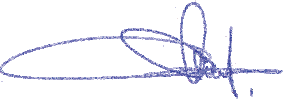
\includegraphics{fig/sign_ycr.pdf}
\end{minipage}

%\begin{minipage}\end{minipage}

%\fig{slm-gamma}{532 nm}
\clearpage

\appendix
\appendixpage
\addappheadtotoc


\chapter{Hologram Generation Matlab Algorithms}
\fig{h}{Schematic representation of the hologram generation}
Figure \ref{algos} shows the inputs and the outputs of each algorithm. The target is sparse matrixes containing the position of the different traps are passed to the hologram generation function. A complex value is used to move the trap in the z-axis while the magnitude is related to the trap intensity, normalized to 1. \texttt{scale\_target} is a two values array indicating the size of the target. \texttt{size\_hologram} give the dimensions in pixels of the output hologram and \texttt{pixel\_hologram} refers to the hologram pixel size. 
\label{algos}


For batch processing, each algorithm can be called with the same function with: 
\begin{lstlisting}
% Algorithms 
ALG = {@RM, @S, @SR, @GSW}; ALG_name = {'RM','S','SR','GSW'}; 

% Build the Holograms
holoSize = [p.slm.height, p.slm.width]; holoPix  = p.slm.pixel_size;

Build = @(target, fun) fun(target, p.scale_target, holoSize, holoPix, p.wavelength, p.setup.fl);

% Exemple of use
Target = sprand(100,100,0.1);  % Random traps distribution
Hologram = Build(Target, @SR); % Hologram computation 
\end{lstlisting}
\clearpage
\section{Random Mask}
\label{rmsource}
This random mask implementation has no loops which is preferred with Matlab. A matrix $R$ contain a random matrix containing an existing trap number. The hologram $H$ is generated by taking the phase value for each corresponding trap. 
\vfil

\lstinputlisting{matlab/rm.m}
\clearpage
\section{Superposition and Random Superposition}
\label{srsource}
\subsection{Matlab}
The SR algorithm can be implemented without loop but in this case, the computing speed and the used memory are more reasonable. A loop will superpose the hologram of each single trap and the composant \texttt{rand(1)*2*pi} is the only difference between the S and the SR algorithm. 
\vfil
\lstinputlisting{matlab/sr.m}
\clearpage
\subsection{GLSL}
\label{glsl}
This is the OpenGL implementation of a pixel shader. Uniforms passed to the shader are \texttt{SX} and \texttt{SY} the position of each trap. \texttt{AC} is the number of active traps and \texttt{W} and \texttt{H} are the real size of the hologram. For compatibility reasons, it is not possible to dynamically adjust the size of \texttt{MAXNUMBERTRAPS}. This parameter has to be specified during the compilation. This means this current implementation is limited for a maximum of 20 traps. At the end, the pixel color is returned in $\texttt{gl\_FragColor.rgb}$. 

\lstinputlisting{matlab/sr.glsl}

\clearpage
\section{Weighted Gerchberg-Saxton}
\lstinputlisting{matlab/gsw.m}

\chapter{List of the Equipment used}

\section{Opto-mechanical elements}
{\small
\begin{tabularx}{\textwidth}{|p{5cm}|X|c|} \hline
\textbf{Model} & \textbf{Description} & \textbf{Serial} \\ \hline
Zeiss SteREO CL1500 ECO & 150W Hallogen light source & - \\ \hline
Zeiss 518F & Immersion Oil ne=1.518 & - \\ \hline
Coherent Sapphire CW CDRH & Laser 488nm 100mW & LDP.1154754.136047 \\ \hline
Thorlabs PM300 & Dual Channel power meter & - \\ \hline
Andor X-600 & Camera & X-6493/C6440 \\ \hline
Allied GE1650 & Camera 1600x1200 & 02-207SC-06143 \\ \hline
\end{tabularx}}
%\end{sideways}
\section{Electronic elements}

%\chapter{Pluto Holoeye softwares}
%\fig{holoeye-voltages}{}

\chapter{Custom mechanical parts}
\section{Hologram Holder}
\begin{center}
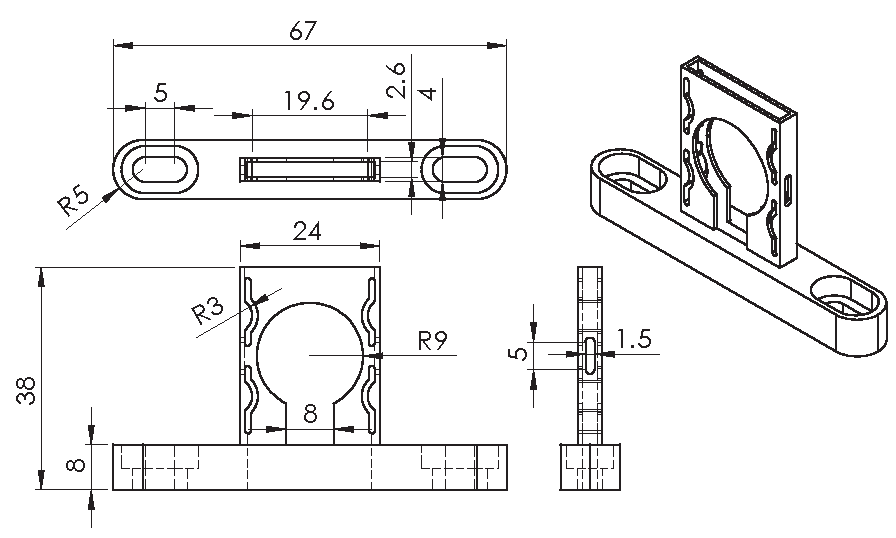
\includegraphics{fig/drwg-hologram.pdf}
\end{center}
\clearpage
\section{Calibration Mask}
\begin{center}
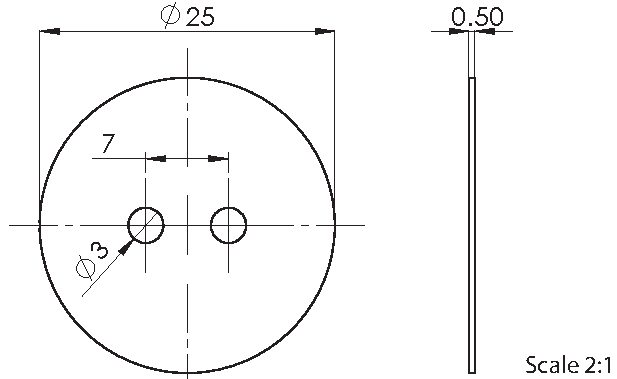
\includegraphics{fig/mask.pdf}
\end{center}
\section{Light source holder}
\label{partlight}



\chapter{Practical tricks}
\section{Telescope alignment}
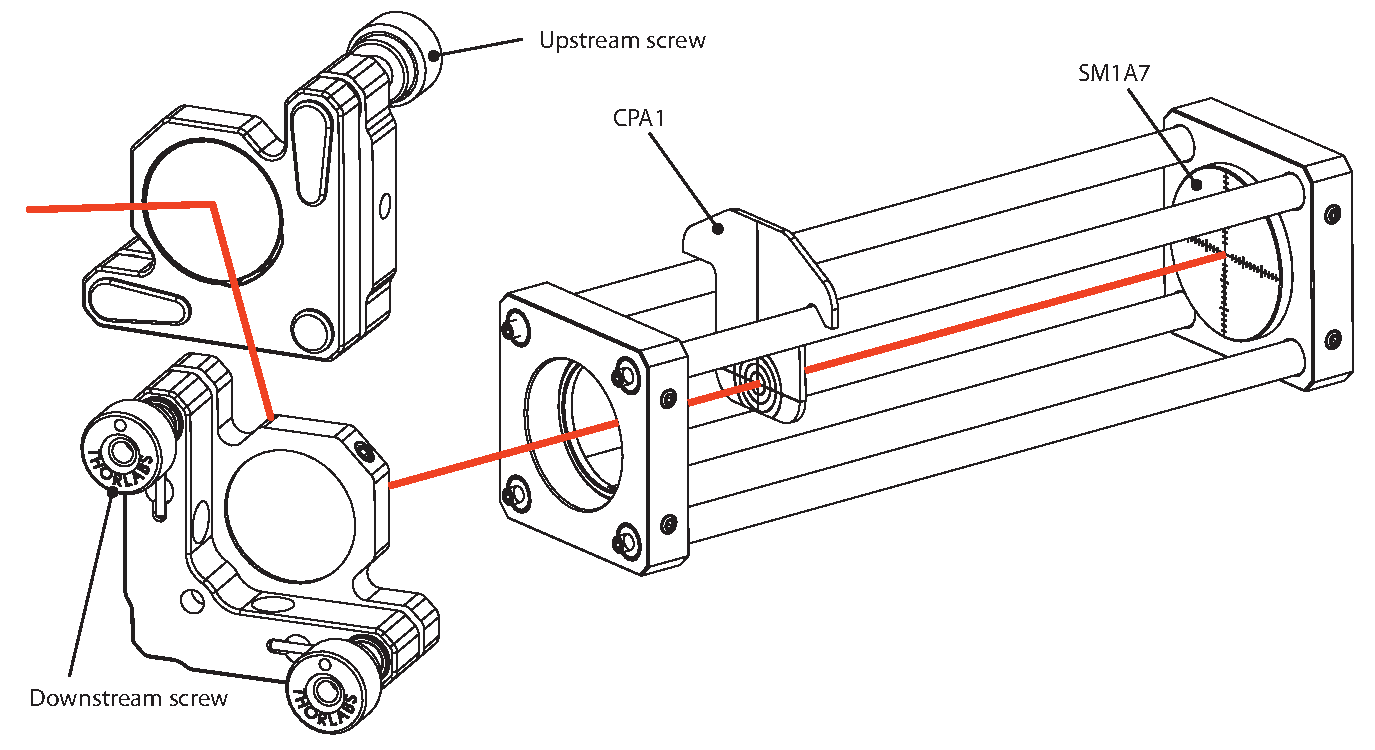
\includegraphics[width=\textwidth]{fig/alignment1.pdf}
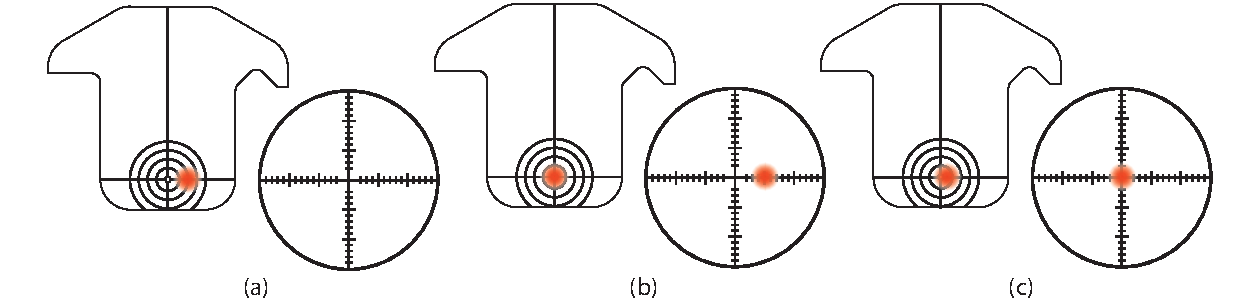
\includegraphics[width=\textwidth]{fig/alignment2.pdf}

\section{1951 USAF Target}
The 1951 USAF resolution test chart is a resolution test pattern set by US Air Force in 1951. It is a common resolution pattern in optics. The microscope versions are chromium coated on a glass substrate. It exists a positive and a negative version in Thorlabs. Both offer a resolution down to 288 line per millimeter.  
\subsection{Find the smallest group}
It is always tough to find the smallest group when used with a high magnification objective. However, a method allows to considerably reduce the time spent. Firstly, we notice the block numbers are always located at the side of horizontal lines (a) and the group numbers are located above vertical (b) or horizontal lines (c). Secondly we notice a smaller pattern is always located at a vertical position that is in between the block numbers 3 and 4 (d). 

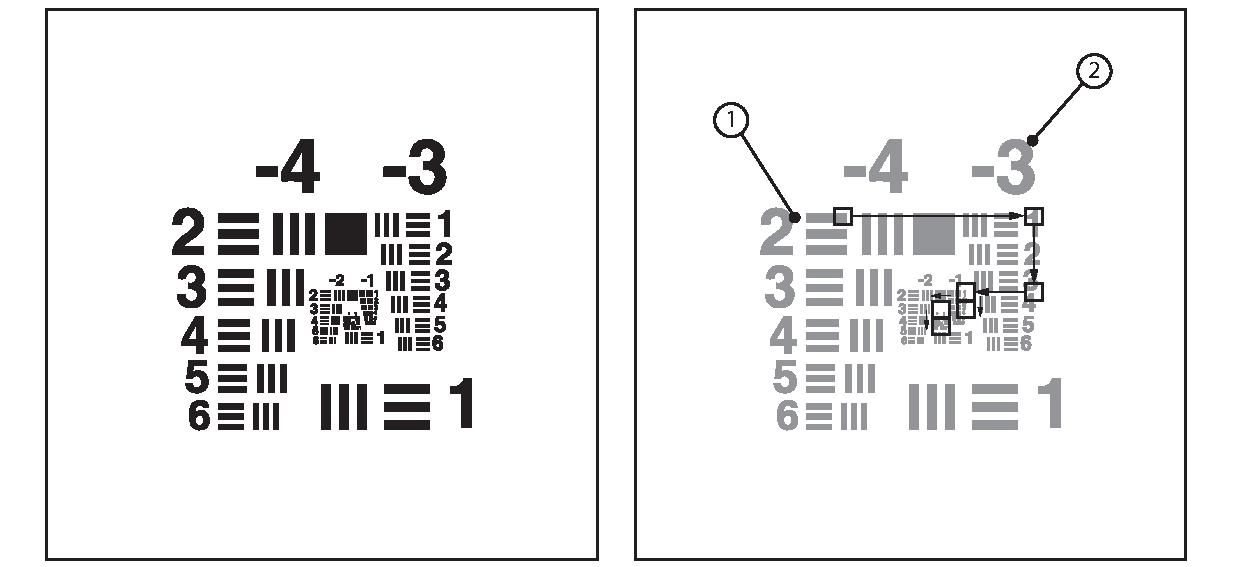
\includegraphics[width=\textwidth]{fig/1951.pdf}

\includegraphics[width=\textwidth]{fig/1951-2.pdf}

Here we randomly started on the edge of the the top horizontal line group -4 block 2. By moving on the left we notice there is number, too big to be seen. It is obviously a block number. By moving the target on the right we will find the opposte block number belongs to a smaller group. Here we can read 1 then we go down to a position between 3 and 4 and we move left again to find the smaller pattern. Again we find the 3 and 4 until we find the smaller group.
\clearpage 
\subsection{Obtain group size and resolution}
The documentation that come with the targets are usually not very clear. The notion of line-pair should called instead spatial period.\par 

\includegraphics[width=\textwidth]{fig/1951-3.pdf}

The resolution in periods per millimeters (line-pair/mm) is given by: 
\begin{equation}
R = 2^{\rm{group}+(\rm{element}-1)/6} 
\end{equation}

A line of width $w$ is therefore given by:
\begin{equation}
w = \frac{1}{2R} = \frac{1}{2^{\rm{group}+(\rm{element}-1)/6}}
\end{equation}
 
And a whole block has a length $L$ of:
\begin{equation}
L = \frac{5}{2R} = \frac{5}{2^{\rm{group}+(\rm{element}-1)/6}}
\end{equation}

\subsection{Target orientation}
A glass coated target is often used in the wrong way. It has to be used in the coated side. By observing the orientation of the group and element numbers and the side of the resolution target it is possible to make sure the orientation is correct. 
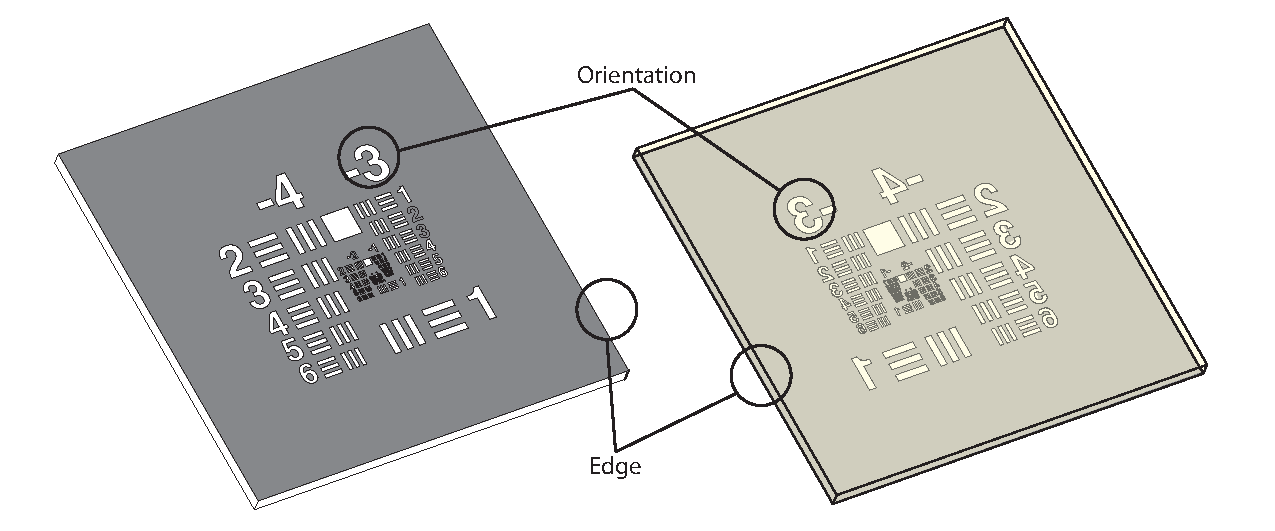
\includegraphics[width=\textwidth]{fig/1951-4.pdf}

\chapter{Experimental setup pictures}
\section{Hologram Holder}
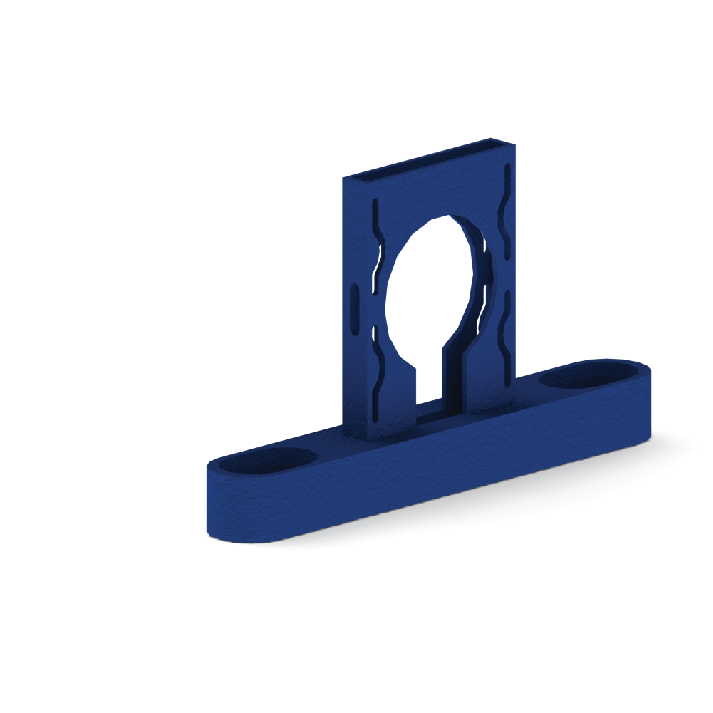
\includegraphics{fig/3d-holo.pdf}
\section{Calibration setup}
\fig{slm-setup3D}{3D view of the setup}
\backmatter

\bibliographystyle{plain}
\bibliography{biblio}

\listoffigures
\listoftables

\makeglossaries
\printglossaries

\printindex

\clearpage
\Large\textbf{Colophon:}\par\normalsize
\thispagestyle{empty}
The quality of this document returns to the outstanding text engine, \LaTeX. The page layout and formatting are inspired from the O'Reilly book entitled \emph{Version Control with Subversion}. 

All the diagrams and illustrations in this report were created with Adobe Illustrator CS5, SolidWorks 2012 and Matlab. All the figures were converted in PDF files. 

This document was compiled with pdflatex and bibtex using Vim and vim-latex. The references was managed with JabRef 

The typefaces in this document are Computed Modern created by Donald Knuth with his METAFONT program. 
\vfil
\begin{center}

\includegraphics[width=5cm]{fig/ctanlion.pdf}
\end{center}
\vfil

\includegraphics[width=5cm]{fig/qr2.pdf}
\end{document}

%vim: set spell:

 

